%% ----------------------------------------------------------------
%% Thesis.tex -- MAIN FILE (the one that you compile with LaTeX)
%% ---------------------------------------------------------------- 

% Set up the document
\documentclass[a4paper, 11pt, oneside]{Thesis}  % Use the "Thesis" style, based on the ECS Thesis style by Steve Gunn
\graphicspath{Figures/}  % Location of the graphics files (set up for graphics to be in PDF format)

% Include any extra LaTeX packages required

\usepackage{verbatim}  % Needed for the "comment" environment to make LaTeX comments
\usepackage{vector}  % Allows "\bvec{}" and "\buvec{}" for "blackboard" style bold vectors in maths
\usepackage[utf8]{inputenc}
\usepackage{subfiles} % access files in subdirectories
\usepackage{tabularx}
\usepackage{float}
\usepackage{amsmath}
\usepackage{csquotes}
\usepackage{listings}
\usepackage{fixltx2e}
\usepackage[english]{babel}
\usepackage{comment}
\usepackage{tikz}
\usepackage{hyperref}
\usepackage{glossaries}
\usepackage{graphicx}
\usepackage{subcaption}
\usepackage{pdfpages}
\usepackage{appendix}

\usepackage[
backend=biber,
style=ieee,
maxbibnames=120
]{biblatex}
\newcommand{\bibdirectory}{01_initial_try.bib}
\newcommand{\latex}{\LaTeX\xspace}
\newcommand{\tex}{\TeX\xspace}

%glossary making
\makeglossaries
% Example:
%\newglossaryentry{foobar}{%
%  name={Foobar},
%  description={A strange animal, not to be confused with \gls{foo}}
%}


\newglossaryentry{vector}{
    name={vector},
    description={An one-dimensional array of data}
}
\newglossaryentry{hyperparameters}{
    name={hyperparameters},
    description={A model hyperparameter is a configuration that is external to the model and whose value cannot be estimated from data.\parencite{brownlee_what_2017}}
}
\newglossaryentry{nonlinear}{
    name={nonlinear},
    description={The results of a function is unable to be reproduced from a linear combination of the inputs}
}
\newglossaryentry{layer}{
    name={layer},
    description={}
}
\newglossaryentry{InkML}{
    name={InkML},
    description={Ink Markup Language, defined by W3C. \parencite{chee_ink_2011}}
}
\newglossaryentry{WebSocket}{
    name={WebSocket},
    description={Enables event driven communication without. Client and server can push messages.}
}
\newglossaryentry{MVP}{
    name={MVP},
    description={Minimal viable product}
}
\addbibresource{\bibdirectory}
\hypersetup{urlcolor=blue, colorlinks=false, linkcolor=black}  % Colours hyperlinks in blue, but this can be distracting if there are many links.

%% ----------------------------------------------------------------

\begin{document}
\frontmatter      % Begin Roman style (i, ii, iii, iv...) page numbering
% Set up the Title Page
\title  {Recognition of handwritten mathematical symbols and expressions}
\authors {Even Dalen, Håvard Langdal and Torkil Solheim}
\addresses  {\groupname\\\deptname\\\univname}  % Do not change this here, instead these must be set in the "Thesis.cls" file, please look through it instead
\date       {\today}
\subject    {}
\keywords   {}

\maketitle
%% ----------------------------------------------------------------


\setstretch{1.3}  % It is better to have smaller font and larger line spacing than the other way round

% Define the page headers using the FancyHdr package and set up for one-sided printing
\fancyhead{}  % Clears all page headers and footers
\rhead{\thepage}  % Sets the right side header to show the page number
\lhead{}  % Clears the left side page header

\pagestyle{fancy}  % Finally, use the "fancy" page style to implement the FancyHdr headers


%% ----------------------------------------------------------------
% The title page
%\includepdf[width=\textwidth, pages=-, width=\textwidth]{Assets/tittelside.pdf}
    


% The preface page
\preface{
\addtocontents{toc}{\vspace{1em}}  % Add a gap in the Contents, for aesthetics

The assignment was chosen for several reasons. We were curious about handwriting recognition, since solutions typically involves artificial intelligence, machine learning and advanced software engineering. These were fields we all were interested in. We had little to no prior experience with machine learning, and expected this to be challenging. However, this made the assignment more interesting as we were motivated to learn and curious about ways to solve the problems related.

Before choosing the assignment, we read about the basics of neural networks and the mathematics behind them. We quickly understood that a lot of the math we have learned in previous courses was relevant, and being able to make use of this knowledge further increased our interest for the assignment.

Although being exciting, the project included many unknown factors. Learning about machine learning while also trying to build a good product was challenging. From early in the project, we found that cooperation was key in order to be productive. Using an agile mindset and following principles from Modern Agile\cite{agile_modern_????} helped dealing with complex subjects through experimentation and collaboration.

First of all, we would like to thank Ole Christian Eidheim for being both an inspiration and our mentor during this project. We would also like to thank our external mentors Tore Forbregd, Trygve Solstad and Hermund Andre Torkildsen for an exciting project and great inputs.

\vfill

\begin{tabularx}{\textwidth}{XXX}
\includegraphics[width=4cm, trim=0 4cm 0 4cm]{Assets/signatures/even.png} & \includegraphics[width=4cm, trim=0 3.5cm 0 3.5cm]{Assets/signatures/haavard.png} & \includegraphics[width=4cm, trim=0 4cm 0 4cm]{Assets/signatures/torkil_sign.png} \tabularnewline
\centering{$\rule{4cm}{0.15mm}$} & \centering{$\rule{4cm}{0.15mm}$} & \centering{$\rule{4cm}{0.15mm}$} \tabularnewline
\centering{Even Dalen} & \centering{Håvard Langdal} & \centering{Torkil Solheim} \\
\end{tabularx}

\centering{\mydate}\\
\centering{Trondheim}

}

\clearpage  % Preface ended, start a new page

%% ----------------------------------------------------------------
% The Assignment page
\assignment{
\addtocontents{toc}{\vspace{1em}}  % Add a gap in the Contents, for aesthetics
\label{assignment_page}
%Erfaring viser at oppgavetekster endres underveis. Dere kan lime inn oppgaveteksten slik den var opprinnelig dersom det fortsatt er i samsvar med virkeligheten. Ellers gjør derekort rede for oppgaven slik den opprinnelig var,og slik den har utviklet seg underveis. Hvorfor ting har blitt som de har blitt, hører kanskje hjemme lenger ut i rapporten –det kommer litt an på hva det er.

\textit{
In this project, a system for recognizing handwritten mathematical symbols will be developed. The system will be used in a web application, Matistikk, that is being developed at the Department of Teacher Education in collaboration with IDI. The system will use a standard machine learning algorithm such as convolutional neural networks that represent state-of-the-art handwriting recognition. Training data must be collected from students to train the network.
}

Since the beginning of the project, some changes were made to the assignment. In the initial phase it was not known if developing a system that would work well and enrich the functionality of the web application was actually achievable. It was therefore decided to go in the direction of developing a proof of concept, which could be developed further.

After some discussion with our mentor, the project was also limited to focus on the handwriting recognition system, and not how to implement it into the web application. Creating a robust and acceptable system would require a lot of work. In addition, with no prior experience with machine learning, a considerable amount of time would be needed to research relevant topics and read about existing solutions. 

}
\clearpage % Assignment ended, start a new page 
%% ----------------------------------------------------------------
% The Abstract Page
\abstract{
\addtocontents{toc}{\vspace{1em}}  % Add a gap in the Contents, for aesthetics

In this thesis we researched different approaches for recognizing handwritten mathematical symbols and expressions. Interpreting different typographic styles has historically been a challenging task, however, recent improvements in both hardware and software for machine learning have made the task more approachable.

The purpose of the assignment was to create a module which interprets mathematical symbols and expressions. We created an example system to display how our module can be integrated into an independent system. Combined, the module and example system provide the complete functionality as specified by our project owners. 

Through our research, we explored different methods in pre- and post-processing of digital handwriting in order to best classify mathematical expressions. Our two approaches were to process drawings into images (using convolutional networks) and interpreting raw trace data (using recurrent networks). The combination of both approaches gave the best result and is the architecture used in our final model.
}

\clearpage  % Abstract ended, start a new page
%% ----------------------------------------------------------------

\setstretch{1.3}  % Reset the line-spacing to 1.3 for body text (if it has changed)

\pagestyle{fancy}  %The page style headers have been "empty" all this time, now use the "fancy" headers as defined before to bring them back


%% ----------------------------------------------------------------
\lhead{\emph{Contents}}  % Set the left side page header to "Contents"
\tableofcontents  % Write out the Table of Contents

%% ----------------------------------------------------------------
\lhead{\emph{List of Figures}}  % Set the left side page header to "List if Figures"
\listoffigures  % Write out the List of Figures

%% ----------------------------------------------------------------

%% ----------------------------------------------------------------
%\setstretch{1.5}  % Set the line spacing to 1.5, this makes the following tables easier to read
\clearpage  % Start a new page


\addtocontents{toc}{\vspace{2em}}  % Add a gap in the Contents, for aesthetics


%% ----------------------------------------------------------------
\mainmatter	  % Begin normal, numeric (1,2,3...) page numbering
\pagestyle{fancy}  % Return the page headers back to the "fancy" style

% Include the chapters of the thesis, as separate files
% Just uncomment the lines as you write the chapters


% TODO; Make sure that the subdirectory can be compiled.
%\subfile{Chapters/Chapter1_Introduction}
\chapter{Introduction}
\lhead{\emph{Introduction}}  % Set the left side page header to "List if Figures"

\section{Motivation} % needs restructuring, we are finding out a way to combine cnn and rnn's, not develop 
% proof of concept++++++

In education, the usage of digital tools has increased. 

%static input system
%preferable with more dynamic input
%more freedom to the student
%the student can show their thoughts in a more precise way (?)
%Something about matistikk

%Some of these tools uses a static system to let the students answer tasks, such as Matistikk, which is a web application for practising math. The main


In education the usage of digital tools to present and distribute tasks to students has increased [0]. % trenger kilde

This includes tasks with multiple choice, graphs, geometric models and algebra. Traditionally these tools does not support dynamic input in form of digital ink, which makes the tools somewhat unrealistic from classic math on paper. \\
%To compensate for a static 

% this needs data to backup my statements
\\ % FUCK JEG TRENGER FAKTA! %Matistikk does have Geogebra integration which is working as intended, but a model for interpreting handwritten math is desired because it would, if implemented in a right way increase the efficiency for both the teachers and the students.
\section{Problem definition} % TODO review if this is actually somehting that we can find out etc...% 1st draft
How can proportionality and relativity be used in recurrent neural networks? \\ Our problem was created after being presented with our project task, which is a task to create a module for interpreting handwritten mathematical symbols. The task itself was focused on creating an generic module which could easily be used in both existing and upcoming projects for the department of teacher education at Norwegian University of Science and Technology. \\ \\
%Eventually the project came to a crossroad between creating a module which were to serve 


\section{Structure of the report}
\subsection{Chapter 1 Introduction}
The introduction introduces important thoughts, concepts and motivation behind this project without going in depth.

All of the concepts introduced in this chapter are required to understand both relevance and motivation.

\subsection{Chapter 2 Theory}
The theory consists of relevant theory to understand both approach, limitations, choices and eventually conclusion.\\
By our project definition we are to expect that the reader is at a level of a 2nd year computer engineering student at our own department. \\
Even though we know that the 2nd year computer engineering student does have the conceptual knowledge required to understand the theory behind neural networks, some of the mathematics will be explained.

\subsection{Chapter 3 Method}
This chapter has a direct correlation with chapter two. Here the choices and technology in chapter two are justified.\\
In addition, we will also discuss tools that made our project flow optimal. \\

% IS THIS RIGHT? % "Referansearkitektur????"
% Some algorithms, general domain model......

\subsection{Chapter 4 Results}
The results are divided into at least three parts. \\
\begin{enumerate}
    \item Scientific results
    This section will describe the data/product which will serve as a foundation for answering our problem/hypothesis in chapter 1.1.
    
    \item Engineering results
    This section will describe the goals set in the start of this project. In a clearly defined product and goal this would be the vision document, in this projects case it would be much more up to the external mentors. %??
    
    \item Administrative results
    This section will go into the process behind this project, from the planning stage to the finishing touches on the thesis. In addition to the process we will also talk about our goals set early in the project phase, and how our goals changed according to our progress and knowledge. Eventually we will arrive at methodology and how there was made attempts to follow agile methodologies.
    
\end{enumerate}

\subsection{Chapter 5 Discussion}
The discussion is also divided into the same parts as Chapter 4. % TODO eholde hvem?
In this chapter we are to answer some questions.
%Why, or why didn't or hypothesis hold?

To explain the different sections, the questions linked to each section is listed underneath.
\begin{enumerate}
    \item Scientific results
    Why did, or why didn't our hypothesis or scientific problem hold?
    In addition to discussing the hypothesis we are to discuss how our results can be interpreted in combination with or as an answer to our hypothesis or scientific problem.
    
    \item Engineering results
    How did the software part of this project turn out? Were the external mentors satisfied with the result? Which requirements were met and which were not? Why did the results become what they are? What went good? What went bad?
    
    \item Administrative results
    What went good or bad as a result of choosing a specific process, approach or technology? What went good or bad regardless of the chosen process, method or technology?
    
\end{enumerate}

% TODO Svakheter => samfunn => etikk => miljø ...
% avsnitt som reflekterer over gruppearbeidet
% 
In addition to discussing our results, the weaknesses of this work should is to be discussed, how it could have been done differently and so forth. 

\subsection{Chapter 6 Conclusion}
The purpose of this work is to find ways of how to use machine learning to recognize handwritten mathematical symbols. Our external mentors have a need, and our goal is to fulfill that need in the best way possible. We hope to accomplish exactly that by examining the different approaches to an issue like this and try to achieve desired results.\\
In addition to the project 

\subsection{Attachments}

\section{Target audience}
% INTRODUSERE TARGET AUDIENCE
%Even though machine learning is a hot topic these days, we encourage the reader to be open to some of the technical aspects in which we hope to present you with. 


\subsection{Report} % Er dette et godt ord??
This project report is meant for everyone curious about an specific introduction to practical examples of machine learning using neural networks. The specific part is linked to this projects assignment, which is to use different approaches to achieve an respectable accuracy.\\
% line break
Even though this report is meant as an introduction to a complicated field, we have based our writing on that the reader has knowledge equivalent to an 2nd year computer engineering student at Norwegian University of Science and Technology in Trondheim. Thus, some of the fundamentals are excluded. % ok setning?


\subsection{Application}
The application which consists of an simple back end and a front end library is available to use under the MIT license. As previously stated, the application is specifically created to fit the needs of our external mentors, but the front end library can be used in a more general matter. % TODO bruk bilder, figurer eller lignende av applikasjonen (?)


\section{CROHME}
CROHME is an abbreviation for Competition on Recognition of Online Handwritten Mathematical Expressions, this competition inspired our work and provided both tools and data for research purposes.\\
The data provided by CROHME was sequential data in a format specified by W3C, called InkML. %https://www.w3.org/TR/InkML/
%InkML is a format well suited for supervised learning, we had our sequential data and a label or truth.\\

% TODO legg inn litt eksempel på inkml (Sekvensiell data)

\section{Purpose}
% Interpret mathematical symbols and expressions and figure out how rnn/cnn/... can be used to obtain desirable accuracy

%\section{Cooperation with the department of Teacher Education, NTNU}
% Owners of matistikk...
% Collection of data (?) and the help we needed to exclude/include some symbols.
The purpose of this project is both to create something useful for our external mentors, while exploring the possibilities and limitations of recognition of handwritten mathematical symbols. In addition to creating something useful, we hope to inspire further work on the subject. Choices made during the project were strongly influenced by previous work, for example \cite{thoma_-line_2015} and \cite{lu_recognition_????}.

\section{Abbreviations}  % Set the left side page header to "Abbreviations"

\begin{tabular}{ l l }
\textbf{ANN} & Artificial Neural Network \\
\textbf{CNN} & Convolutional Neural Network \\
\textbf{CPU} & Central Processing Unit \\
\textbf{CROHME} & Competition on Recognition of Online Handwritten Mathematical Expressions \\
\textbf{GPU} & Graphics Processing Unit \\
\textbf{ILU} & Department of Teacher Education \\
\textbf{InkML} & Ink Markup Language \\
\textbf{JSON} & JavaScript Object Notation \\
\textbf{LSTM} & Long Short-Term Memory \\
\textbf{RNN} & Recurrent Neural Network \\
\end{tabular}



\chapter{Theory}
\lhead{\emph{Theory}}
% TODO CITE
% KERAS
% SKLEARN
% NUMPY

\section{Handwriting recognition}
\label{handwriting_recognition}

Handwriting recognition systems are computer systems that can recognize characters and symbols written by hand. These systems have been continuously developed and researched since the early days of computers \parencite{simon_off-line_1992}, beginning with the optical character recognition (OCR) systems in the 1950s \parencite{mori_historical_1992}. The early OCR systems were very limited in terms of hardware, which resulted in slow progress. Researchers had high aspirations for handwriting recognition, however, it quickly gained the reputation of being an extremely difficult problem \parencite{simon_off-line_1992}. As hardware and computers became more advanced, the OCR and handwriting recognition systems followed in the same direction. However, hardware has often been a bottleneck for these systems. \parencite{mori_historical_1992}

When computational power increased, using artificial neural networks became more popular, also for handwriting recognition. For example, in \cite{fukushima_handwritten_????} by Fukushima et al., a neural network was trained to recognize 35 symbols. Since then, neural networks has been used in many solutions, and has proven to be a major contributor to the field, as it is one of the most used tools in leading solutions today (some of these are presented in section \ref{previous_work_existing_solutions}).

This field has for a long time been a worldwide research project \parencite{mori_historical_1992}, and many competitions on different handwriting recognition problems has been arranged. Researchers from all over the world has cooperated to produce various solutions, which further confirms the difficulty of a general handwriting recognition system. 

\subsection{Main approaches}
\label{main_approaches}

Handwriting recognition systems generally has two main approaches, online and offline \cite{priya_online_2016}. Online recognition uses data from pen strokes based on sampled coordinates of pen movements and the time difference between them. These pen strokes are also referred to as traces.  Each trace can be uniquely identified while drawing, which in many cases can aid in the segmentation problem (see section \ref{Segmentation}).

While online recognition uses sequential data, offline recognition uses images. In this approach the recognition system relies solely on the pixel values in images. Traces can therefore not be uniquely identified, as opposed to online recognition

%In offline recognition, traces cannot be uniquely identified, as opposed to online recognition.

\begin{figure}[H]
\centering
\begin{subfigure}{0.3\textwidth}
\includegraphics[width=1.1\linewidth, height=5cm]{Assets/Chapter2_Theory/segmentation_2_on.png} 
\caption{}
\label{fig:online_data}
\end{subfigure}
\begin{subfigure}{0.3\textwidth}
\includegraphics[width=1.1\linewidth, height=5cm]{Assets/Chapter2_Theory/segmentation_2.png}
\caption{}
\label{fig:offline_data}
\end{subfigure}
\caption{A: Online input data with coordinate samples. B: Offline input data (only an image).}
\label{fig:online_offline_comparison}
\end{figure}

With the online input data, creating images of the traces is possible by drawing lines between the coordinates. This means that online recognition systems has access to roughly the same images as offline recognition systems, in addition to the coordinates. Having more features to analyze is important since handwriting styles can vary a lot. In general, online recognition systems has higher performance and accuracy than offline recognition systems \parencite{priya_online_2016}.

\subsection{Common steps in handwriting recognition}

In the recognition process there are several problems that must be solved. Usually, the most common problems include segmentation and classification of symbols. In addition to these steps, the pre- and postprocessing might include complicated algorithms.

\subsubsection{Preprocessing}

In the preprocessing step the raw input data is prepared for analysis. Raw input data can come in many formats and sizes, and may contain values that are not valid. This step deals with these problems and converts the data to a format that suits the consecutive steps better. To further optimize the flow, excess data can be discarded.

It is also important to discard excess data to avoid misinterpretations \parencite{huang_preprocessing_2007}.

A common task in preprocessing is to normalize the input data. This simply means that all the data is scaled to the same value range and is cleaned for values that are not valid. For handwriting recognition, normalizing generalizes the different writing styles by removing some of the variations \parencite{huang_preprocessing_2007}.

Since the input can be offline or online, there are many techniques that can be used to prepare the data. Common tasks in preprocessing of offline data includes removal of noise from the images and converting greyscale images to binary images \cite{priya_online_2016}. The images could also be scaled and modified to not contain any blank or empty space.

Online data can be processed in different ways than offline data. For example, the coordinates can be plotted and lines can be drawn between them. This is often called a polygonal chain. Without any preprocessing these plots can have sharp edges and overall be a inaccurate representation of handwriting. Smoothing could be applied to the coordinates to fix this by using interpolation of points. The data samples might also need to be parsed to a format that is more suitable for processing, such as matrices or arrays.

To normalize traces to have the same number of data points, a variation of the Ramer-Douglas-Peucker (RDP)\cite{h_algorithms_2011} algorithm can be used. The RDP algorithm attempts to simplify a polygonal chain, while minimizing the difference between the original and the simplified chain. The simplification process works by finding data points which influences the shape of the polygonal chain less than a fixed threshold.

The algorithm can be modified to decrease the number of data points to a fixed number. This can be done by iterating all the data points three at a time, and removing the middle point with lowest perpendicular distance to a line drawn between the two endpoints.

\begin{figure}[H]
    \centering
    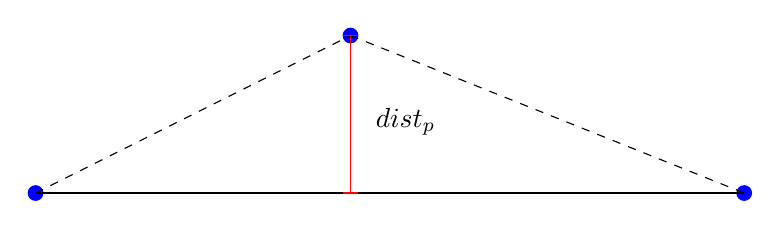
\begin{tikzpicture}
    
        %Datapoints
        \fill[blue] (-3, 0) circle (0.1cm);
        \fill[blue] (1, 2) circle (0.1cm);
        \fill[blue] (6, 0) circle (0.1cm);

        \draw[-] (-3, 0) -- (6, 0);
        \draw[dashed] (-3,0) -- (1, 2);
        \draw[dashed] (1, 2) -- (6, 0);
        
        \draw[red, -] (1, 2) -- (1, 0);
        \draw[red, -] (0.9, 2) -- (1.1, 2);
        \draw[red, -] (0.9, 0) -- (1.1, 0);
        \node at (1.7, 0.9) {$dist_p$};

    \end{tikzpicture}
    \caption{Figure of calculating the perpendicular distance to a line drawn between two endpoints}
    \label{fig:my_label}
\end{figure}
\label{ramer_douglas_peucker}

In order to normalize traces from different sources, their coordinates needs to be scaled within the same range. A maximum and and minimum value, the roof and floor of the range specified, is used together with a list of x- or y-coordinates.

First, the maximum and minimum values of the list is found, as well as the difference between them. The scaled values is then found with this formula:

\begin{equation} \label{eqn:scale_linear_by_column}
\centering
\begin{split}
    s = roof - \frac{(roof - floor) \cdot (max(x) - x)}{diff}
    %CITE THIS SHIT WITH GIST
\end{split}
\end{equation}


\label{scale_linear_by_column}
% CITE: https://gist.github.com/perrygeo/4512375

\subsubsection{Segmentation} \label{Segmentation}

The segmentation problem deals with extraction of symbols from trace-coordinates or images. Deciding if two traces that overlap belongs to the same symbol is difficult, since they can overlap in countless ways. 

\begin{figure}[H]
\centering
\begin{tikzpicture}
\begin{scope}[xshift=1.5cm]
    \node[anchor=south west,inner sep=0] (image) at (0,0) {\includegraphics[width=0.2\textwidth]{Assets/Chapter2_Theory/segmentation_2.png}};
    \begin{scope}[x={(image.south east)},y={(image.north west)}]
        \draw[->] (1,0.5) -- (1.9,0.8);
        \draw[->] (1,0.4) -- (1.9,0.4);
        \draw[->] (1,0.3) -- (1.9,0);
        \node [anchor=west] (note) at (2,0.9) {\Large 2x};
        \node [anchor=west] (note) at (2,0.4) {\Large $\Delta$};
        \node [anchor=west] (note) at (2,-0.1) {\Large 2/\textbackslash};
        \node [anchor=west] (note) at (2.4,0.4) {\Huge ?};
    \end{scope}
\end{scope}
\end{tikzpicture}
\caption{The segmentation problem deals with extraction of symbols from trace-coordinates or images. The sample above has three traces, one for the "2"  and two for the "x". How they are segmented can lead to many different outcomes.}
\label{fig:segmentation_1}
\end{figure}

Correctly segmenting the symbols plays a big role in the recognition process since it heavily affects the final results. A simple way of dealing with the problem with online data is to merge the traces that overlap to a single symbol. In this case the sample above would combine the '2' and the 'x' to a single symbol, which would lead to a wrong classification. A more complicated approach is presented in \cite{nguyen_improved_2015} where bidirectional long-short term memory neural networks (see section \ref{theory-LSTM}) is used to segment English handwritten text.

\subsubsection{Classification of symbols}
The classification step deals with the actual recognition. In this step each of the segmented symbols is classified to a truth. All these different truth values builds up an alphabet and is the vocabulary that the system understands. As the size of this alphabet increases, the recognition rates typically drops since the system has to distinguish between more types of symbols. Some of these symbols could also look similar, such as the numbers 1 and 7. 

%A popular approach for this is to use neural networks (see section \ref{artificial_neural_networks}). For image classification, neural networks has achieved very high rates and is regarded as the current state-of-the-art [KILDE].

\subsubsection{Postprocessing}

After the classification the results can be further analyzed and converted to the desired format. In \cite{hu_research_2011} a dictionary based postprocessing method is used to improve the recognition results by checking if the classification results is valid. With a dictionary the recognition system can filter out words that does not exist, and replace them with similar and valid words. Another way to further improve the results is to use contextual analysis. With this approach the positions of the input data is analyzed with regards to the classification results. Grammatical errors and results that does not make sense might be revealed, and can be used to trigger a re-classification with the last results in mind.


\section{Recognition of handwritten mathematics} 
\label{recognition_of_handwritten_mathematics}
Recognition of handwritten mathematics is a field in handwriting recognition that deals with mathematical symbols and expressions. This field shares many of the same problems as recognition of words and characters, however, there is also a new problem that must be dealt with. Just as regular language, mathematics has a set of grammatical or positional rules that should be followed. For example, there are fractions, exponents and square roots that has to be interpreted correctly. This two-dimensional notation requires further processing techniques compared to analyzing regular words.

A context of how all the symbols fit together has to be built by looking at positional values. This context search could be done in the post-processing step, using the results of the classification for guidance. The classification of symbols might also be completely wrong, as the truth to a symbol has many context-dependencies \cite{zanibbi_recognition_2012}. For instance, the decimal separator "." and the multiplication operator "$\cdot$" must be interpreted based on their position to their surroundings.

%\begin{figure}[H]
%  \centering
%  \label{steps_in_math_recog}
%\end{figure}
%[Image of the steps in math recog]

\subsection{Previous work and existing solutions}
\label{previous_work_existing_solutions}
There is a lot of work previously done in recognition of handwritten mathematics, and many solutions has been made. The first work in this field dates back to the 60s and has gradually developed since \cite{mouchere_icfhr2016_2016}. Different solutions and ideas has been presented through many publications from all over the world. For example, in \cite{matsakis_recognition_????} from 1999, a system that uses a Gaussian classifier for recognition of handwritten mathematics is demonstrated.

In recent years a competition called Competition on Recognition of Online Handwritten Mathematical Expressions hosted by ICFHR has been held \cite{mouchere_icfhr2016_2016} \cite{mouchere_advancing_2016}. In these competitions teams from around the world competed in various math recognition tasks. The main task was to recognize expressions, while subtasks for example was to recognize matrices and isolated symbols. This competition has contributed a lot to the math recognition field, by producing standardized data sets and evaluation metrics.

In the CROHME competition held in 2016 the MyScript corporation won in all categories. To produce the best results, their system handles segmentation, classifying and interpretation concurrently. The system uses features from both bitmaps and digital ink traces that is sent through a combination of MLP and recurrent neural networks \cite{mouchere_icfhr2016_2016}. As of \mydate their technology is commercially available.

\subsection{InkML}
InkML is a markup language based on XML to describe digital ink data. The format is specified by the World Wide Web Consortium (W3C) \cite{chee_ink_2011}. InkML groups it's content in specific XML-style elements called ink. These elements contains trace elements, which stores coordinates for the traces. 

%the ink element often has sub elements which is a trace element.\\

\begin{figure}[H]
\begin{lstlisting}[language=XML]
<trace id="0">
    207 136, 199 141, 197 143, 196 144, 195 146, 194 147, 193 149
</trace>
<trace id="1">
    847 201, 847 204, 846 207, 846 211, 846 215, 845 219, 845 222
</trace>
<trace id="2">
    833 235, 822 235, 821 235, 820 235, 819 236, 819 235, 819 236
</trace>

<traceGroup xml:id="3">
	<annotation type="truth">+</annotation>
	<traceView traceDataRef="1"/>
	<traceView traceDataRef="2"/>
	<annotationXML href="+_1"/>
</traceGroup>
\end{lstlisting}

\caption{InkML example of three traces, each with an file-unique id. In addition to traces, a trace group is included to connect truths to traces. Truths are used when providing labels to use in supervised learning, and is explained in section \ref{supervised_learning}.}

\label{fig:InkML_ex}
\end{figure}

\section{Machine learning}
\label{machine_learning}
According to Murphy et al.\cite{murphy_machine_2012}, machine learning can be defined as a set of methods that can automatically detect patterns in data. These uncovered patterns can also be used to predict future data or support decision making. For example, historical data of maintenance can be used to predict failure for individual mechanical parts \parencite{cline_predictive_2017}. Goodfellow et al. explains machine learning as an applied form of statistics. \cite{goodfellow_deep_2016}

\subsection{Supervised learning}
\label{supervised_learning}

Supervised learning is the machine learning task to map an input to an output. It requires large amounts of training data, with features and an additional truth label. 
A supervised learning algorithm could study many examples of what it's going to classify to eventually be able to classify to the correct class. To explain this in another way think of the function p(y $|$ x), this reads the probability of y given x has happened. This is exactly what supervised learning is, where the y labels are provided by a supervisor.

\section{Artificial neural networks}
\label{artificial_neural_networks}

Artificial neural networks (ANN) 
An artificial neural network (ANN) is a network of artificial neurons inspired by biologically neural networks.

ANNs consists of a combination of artificial neurons, also referred to as computational units. These units takes a vector as input. The input is multiplied with the precomputed weights, and a bias is added. A bias is simply a way to change the constant b in equation $y = ax + b$ to shift the equation up or down. Then, the result is summed and used as input to the activation function \ref{activation_functions}. Lastly, the weighted sum is returned as output from the unit. \cite{_cs231n_????} \cite{_multi-layer_????}

\begin{figure}[H]
  \centering
    \begin{tikzpicture}
        \draw[->] (0,2) -- (2.1,0.8);
        \draw[->] (0,0.65) -- (2,0.3);
        \draw[->] (0,-0.65) -- (2,-0.3);
        \draw[->] (0,-2) -- (2.1,-0.8);
    
        \node at (0.2, 2.3) {$x_1$};
        \node at (0.2, 1) {$x_2$};
        \node at (0.2, -0.25) {$...$};
        \node at (0.2, -1.5) {$x_n$};
        
        \draw [] (4.2,0) ellipse (2cm and 1cm);
        
        \node at (4.2,0) {$\sum\limits_{i=1}^{n} W_i \cdot x_i + b$};
        
        \draw[->] (6.5,0) -- (7.5,0);
        
        \draw (7.8, 0.8) rectangle (9.8, -0.8);
    
        \node at (8.8,0) {$f : R \rightarrow R$};
    
    \end{tikzpicture}
    \caption{Diagram of a single artificial neuron. $W_{i}$ is the weight of input edge i, $x_{i}$ is the value coming from edge i and b is the bias.} % TODO denne trenger mer kjøtt, god forklaring fra a til å!
    \label{fig:single_neuron}

\end{figure}

The units in a neural network are typically organized into different layers, where each layer has a fixed number of units. The diagram below is an example of how these units can be connected together.

\begin{figure}[H]
  \centering

    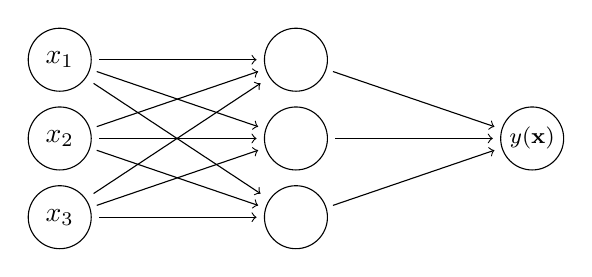
\begin{tikzpicture}
        
        \draw [] (0.5,1) circle [radius=0.4];
        \draw [] (0.5,0) circle [radius=0.4];
        \draw [] (0.5,-1) circle [radius=0.4];

        \draw [] (3.5,1) circle [radius=0.4];
        \draw [] (3.5,0) circle [radius=0.4];
        \draw [] (3.5,-1) circle [radius=0.4];

        \draw [] (6.5, 0) circle [radius=0.4];

        \draw[->] (1,1) -- (3,1);
        \draw[->] (0.97,0.85) -- (3.02,0.15);
        \draw[->] (0.93,0.7) -- (3.05,-0.7);

        \draw[->] (0.97,0.15) -- (3.02,0.85);
        \draw[->] (1,0) -- (3,0);
        \draw[->] (0.97,-0.15) -- (3.02,-0.85);

        \draw[->] (0.93,-0.7) -- (3.05,0.7);
        \draw[->] (0.97,-0.85) -- (3.02,-0.15);
        \draw[->] (1,-1) -- (3,-1);
        
        \draw[->] (3.97,0.85) -- (6.02,0.15);
        \draw[->] (4, 0) -- (6,0);
        \draw[->] (3.97, -0.85) -- (6.02,-0.15);

        \node at (0.5,1) {$x_1$};
        \node at (0.5,0) {$x_2$};
        \node at (0.5,-1) {$x_3$};
        \node at (6.5,0) {\footnotesize$y(\textbf{x})$};

    \end{tikzpicture}
    \caption{Diagram of a neural network with two layers (Output layer and one hidden layer). It contains three units in the input layer, three units in the hidden layer, and a single unit in the output layer. }
    \label{fig:single_layered_neural_network}
\end{figure}


The leftmost layer of units in \ref{fig:single_layered_neural_network} is called the input layer, and is a passive layer. This means that data is not modified in this layer. Each unit in the input layer receives a single input and duplicate the input to its multiple output units. The hidden layer and the output layer from \ref{fig:single_layered_neural_network} are active units. These units modify the data before propagating the values to the next layer (described in \ref{fig:single_neuron}). The result of the output layer is the approximation done by the neural network. \parencite{smith_scientist_1997} 

In order for a neural network to be a good approximator, the weights and biases in each unit has to be optimized to minimize error in the output layer. This tuning process is performed through training. Training a network means giving the network labeled training data, comparing the output label from the network to the label provided, and tuning the weights and biases to best satisfy a loss function (\ref{loss_function}). This optimization process is typically done using an optimizer such as gradient decent, and through a concept called backpropogation. This is described in section \ref{training_with_backpropagation}.

% THIS SECTION IS PREVIOUSLY CALCULATING AN OUTPUT
The output of a neural network is a set of numerical values, one value for each of the output units in the neural network. To create these output values the neural network performs a series of mathematical operations on the input values.
%The output of a neural network is a vector of numerical values. This vector contains as many values as there are output units in the neural network. To create this output vector the neural network performs a series mathematical operations on the input vector. 

For this demonstration the network in figure \ref{fig:single_layered_neural_network} will be used. The first step is to calculate the outputs from the hidden layer, $H_o$.
\begin{figure}[H]
  \centering

    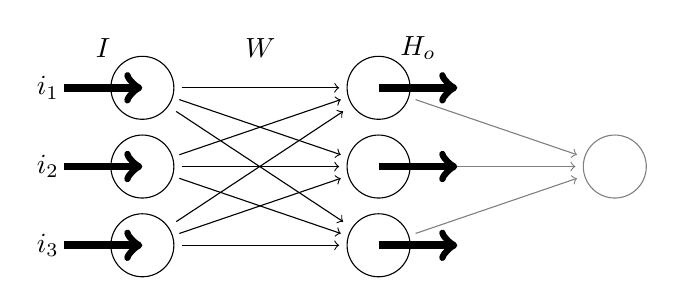
\begin{tikzpicture}
        
        \draw [] (0.5,1) circle [radius=0.4];
        \draw [] (0.5,0) circle [radius=0.4];
        \draw [] (0.5,-1) circle [radius=0.4];

        \draw [] (3.5,1) circle [radius=0.4];
        \draw [] (3.5,0) circle [radius=0.4];
        \draw [] (3.5,-1) circle [radius=0.4];

        \draw [draw={rgb:black,2;white,2}] (6.5, 0) circle [radius=0.4];

        \draw[->] (1,1) -- (3,1);
        \draw[->] (0.97,0.85) -- (3.02,0.15);
        \draw[->] (0.93,0.7) -- (3.05,-0.7);

        \draw[->] (0.97,0.15) -- (3.02,0.85);
        \draw[->] (1,0) -- (3,0);
        \draw[->] (0.97,-0.15) -- (3.02,-0.85);

        \draw[->] (0.93,-0.7) -- (3.05,0.7);
        \draw[->] (0.97,-0.85) -- (3.02,-0.15);
        \draw[->] (1,-1) -- (3,-1);
        
        \draw[draw={rgb:black,2;white,2}, ->] (3.97,0.85) -- (6.02,0.15);
        \draw[draw={rgb:black,2;white,2}, ->] (4, 0) -- (6,0);
        \draw[draw={rgb:black,2;white,2}, ->] (3.97, -0.85) -- (6.02,-0.15);

        %\node at (0.5,1) {$x_1$};
        %\node at (0.5,0) {$x_2$};
        %\node at (0.5,-1) {$x_3$};
        %\node[text={rgb:black,2;white,2}] at (6.5,0) {\footnotesize$y(\textbf{x})$};
        
        \draw[->, line width=1mm] (3.5,1) -- (4.5,1);
        \draw[->, line width=1mm] (3.5,0) -- (4.5,0);
        \draw[->, line width=1mm] (3.5,-1) -- (4.5,-1);
        
        \draw[->, line width=1mm] (-0.5,1) -- (0.5,1);
        \draw[->, line width=1mm] (-0.5,0) -- (0.5,0);
        \draw[->, line width=1mm] (-0.5,-1) -- (0.5,-1);
        
        \node at (0,1.5) {$I$};
        \node at (-0.7,1) {$i_1$};
        \node at (-0.7,0) {$i_2$};
        \node at (-0.7,-1) {$i_3$};
        
        \node at (2,1.5) {$W$};
        \node at (4,1.5) {$H_o$};
        
        

    \end{tikzpicture}
    \caption{The outputs of the hidden layer is calculated based on the inut values and the weights between the input layer and hidden layer.}
    \label{fig:calculating_output_one}
\end{figure}

Each of the input values are multiplied with the weight to each unit in the hidden layer. All the inputs to a unit in the hidden layer is then summed. Matrix multiplication can be used for this, where a matrix containing all the weights is multiplied with a column-matrix containing the input values. The weights matrix in this example is a 3x3 matrix since there are 3 inputs and 3 units in the hidden layer.

\begin{center}
$
W * I = 
\begin{bmatrix} 
w_{1,1} & w_{2,1} & w_{3,1}\\
w_{1,2} & w_{2,2} & w_{3,2}\\
w_{1,3} & w_{2,3} & w_{3,3}
\end{bmatrix}
*
\begin{bmatrix} 
i_1\\
i_2\\
i_3
\end{bmatrix}
=
\begin{bmatrix} 
h_1\\
h_2\\
h_3
\end{bmatrix}
=
H_i
$
\end{center}

To calculate the output from the hidden layer an activation function is used on these input values: $activation(H_i) = H_o$. More details about activation functions is explained in section \ref{activation_functions}.

%\begin{center}
%$
%activation(H_i) = H_o
%$    
%\end{center}

The output from the hidden layer is then sent further in the network.

\begin{figure}[H]
  \centering

    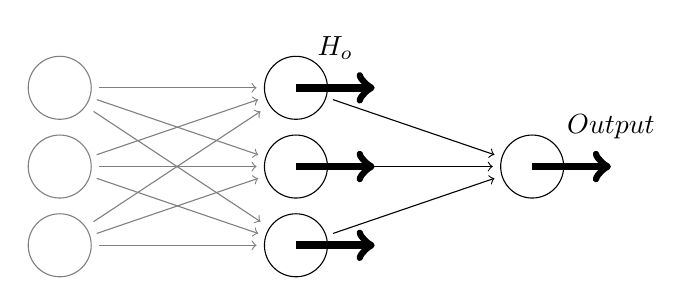
\begin{tikzpicture}
        
        \draw [draw={rgb:black,2;white,2}] (0.5,1) circle [radius=0.4];
        \draw [draw={rgb:black,2;white,2}] (0.5,0) circle [radius=0.4];
        \draw [draw={rgb:black,2;white,2}] (0.5,-1) circle [radius=0.4];

        \draw [] (3.5,1) circle [radius=0.4];
        \draw [] (3.5,0) circle [radius=0.4];
        \draw [] (3.5,-1) circle [radius=0.4];

        \draw [] (6.5, 0) circle [radius=0.4];

        \draw[draw={rgb:black,2;white,2}, ->] (1,1) -- (3,1);
        \draw[draw={rgb:black,2;white,2}, ->] (0.97,0.85) -- (3.02,0.15);
        \draw[draw={rgb:black,2;white,2}, ->] (0.93,0.7) -- (3.05,-0.7);

        \draw[draw={rgb:black,2;white,2}, ->] (0.97,0.15) -- (3.02,0.85);
        \draw[draw={rgb:black,2;white,2}, ->] (1,0) -- (3,0);
        \draw[draw={rgb:black,2;white,2}, ->] (0.97,-0.15) -- (3.02,-0.85);

        \draw[draw={rgb:black,2;white,2}, ->] (0.93,-0.7) -- (3.05,0.7);
        \draw[draw={rgb:black,2;white,2}, ->] (0.97,-0.85) -- (3.02,-0.15);
        \draw[draw={rgb:black,2;white,2}, ->] (1,-1) -- (3,-1);
        
        \draw[->] (3.97,0.85) -- (6.02,0.15);
        \draw[->] (4, 0) -- (6,0);
        \draw[->] (3.97, -0.85) -- (6.02,-0.15);

        \draw[->, line width=1mm] (3.5,1) -- (4.5,1);
        \draw[->, line width=1mm] (3.5,0) -- (4.5,0);
        \draw[->, line width=1mm] (3.5,-1) -- (4.5,-1);
        
        \draw[->, line width=1mm] (6.5,0) -- (7.5,0);
        
        \node at (4,1.5) {$H_o$};
        \node at (7.5,0.5) {$Output$};

    \end{tikzpicture}
    \caption{The final output is calculated}
    \label{fig:calculating_output_two}
\end{figure}
The same process with matrix multiplication and activation function is repeated with the output from the hidden layer and the weights to the output layer. This will calculate the final output from the neural network. Since the output layer consist of only one unit, the final output will be a single value.

For a larger neural network the same process is used but on a bigger scale. If a neural network has more than a single hidden layer, the process is repeated for each of the layers.




\subsection{Activation functions} % TODO  trim dette litt ned, siden core concepts tar for seg basics.
\label{activation_functions}

Activation functions in artificial neural networks has inspiration from how neurons in our brain works. In a mathematical model of an artificial neuron by McCulloch-Pitt \cite{mcculloch_logical_1943}, the activation of a neuron was modelled as the unit step function. This model has later been generalized to use functions such as sigmoid, rectified linear unit, softmax and tangens hyperbolicus. \parencite{jain_artificial_1996}

\begin{figure}[H]
  \centering
    \includegraphics[width=0.9\textwidth]{Assets/Chapter2_Theory/activation_function_overview.png}
    \caption{Three activation functions plotted on the interval [-4,4].}
\end{figure}

One purpose of an activation function is to introduce nonlinearity into the model. A network without nonlinearity can't represent functions which are nonlinear, despite having multiple layers. On the other hand, it is proved that a multilayered feedforward network with nonlinear activation functions can approximate any function (under some constraints). \cite{leshno_multilayer_1993}

 An example of the importance of nonlinearity in neural networks can shown in the exclusive-OR problem illustrated in the figure below. The black dots can not be separated from the white using a single line. On the other hand, a combination of nonlinear functions can create arbitrary shapes to separate the white and black dots. \parencite{jain_artificial_1996} \cite{sharma_understanding_2018}

\begin{figure}[H]
  \centering

    \begin{subfigure}{.45\textwidth}
      \centering

        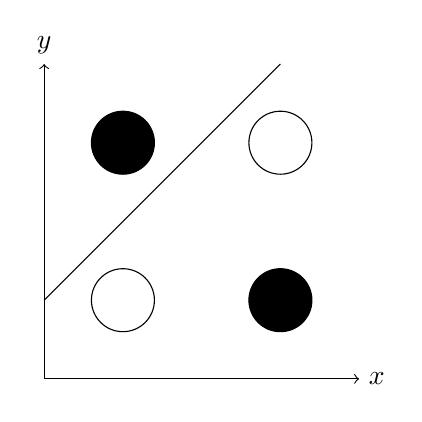
\begin{tikzpicture}
        
            \draw [fill=black] (0.5,1) circle [radius=0.4];
            \draw [] (0.5,-1) circle [radius=0.4];
    
            \draw [] (2.5,1) circle [radius=0.4];
            \draw [fill=black] (2.5,-1) circle [radius=0.4];
    
            \draw[-] (-0.5, -1) -- (2.5,2);
    
            \draw[->] (-0.5,-2) -- (3.5,-2) node[right] {$x$};
            \draw[->] (-0.5,-2) -- (-0.5, 2) node[above] {$y$};

        
        \end{tikzpicture}
        \caption{Using no activation functions}

    \end{subfigure}
    \begin{subfigure}{.45\textwidth}
      \centering

        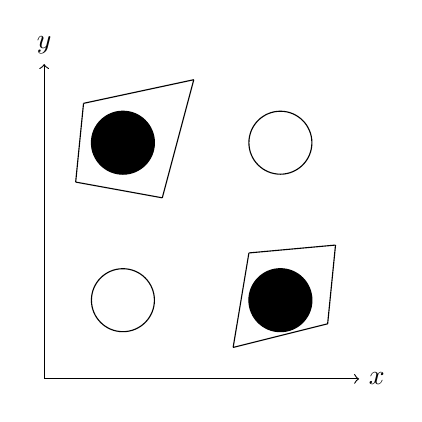
\begin{tikzpicture}
        
            \draw [fill=black] (0.5,1) circle [radius=0.4];
            \draw [] (0.5,-1) circle [radius=0.4];
    
            \draw [] (2.5,1) circle [radius=0.4];
            \draw [fill=black] (2.5,-1) circle [radius=0.4];
    
            \draw[-] (0, 1.5) -- (-0.1,0.5);
            \draw[-] (-0.1, 0.5) -- (1,0.3);
            \draw[-] (1, 0.3) -- (1.4,1.8);
            \draw[-] (1.4, 1.8) -- (0,1.5);
    
            \draw[-] (1.9, -1.6) -- (3.1, -1.3);
            \draw[-] (3.1, -1.3) -- (3.2,-0.3);
            \draw[-] (3.2, -0.3) -- (2.1,-0.4);
            \draw[-] (2.1, -0.4) -- (1.9,-1.6);
    
            
            \draw[->] (-0.5,-2) -- (3.5,-2) node[right] {$x$};
            \draw[->] (-0.5,-2) -- (-0.5, 2) node[above] {$y$};
        \end{tikzpicture}
        \caption{Using non-linear activation functions}% TODO denne kunne trenge mer forklaring
        % TODO verifiser formen på denne? den forrige har linje, men denne har ikke (?)
        % Denne er riktig tegnet, men klassifiseringen må fylles inn, og problemet må forklares bedre
        % Reagerte bare på at den første har linjer og denne ikke. http://www.ece.utep.edu/research/webfuzzy/docs/kk-thesis/kk-thesis-html/node19.html for eksempel.. Bare nysgjerrig

    \end{subfigure}
    
    \caption{Figure of the exclusive-OR problem, by the capabilities of a model with non-linear activation functions versus no activation function.}
    \label{fig:exclusive-OR problem}
\end{figure}

Activation functions are also important for squashing the output of a neural network into desired bounds. A common use case is for returning class probabilities for a classification model, where softmax is often used as the activation function for the last layer. Softmax is an activation function which transforms its inputs to a combined sum of 1. \cite{sharma_understanding_2018}

\begin{figure}[H]
  \centering
    \includegraphics[width=\textwidth]{Assets/Chapter2_Theory/squashin_output_data_using_activation_functions.png}
    \caption{Figure of how example input data is transformed through two different activation functions. Data flows from left to right, with output from the previous graph used as input to the next.}
\end{figure}

\subsubsection{ReLU}

Rectified linear unit or ReLU is a nonlinearity introduced by Hanloser et al. in 2000 \cite{smith_scientist_1997}, and has later been found successful as a nonlinearity in deep neural network. This function disallows negative values, meaning that the output from all negative input values is 0. If the input value is positive, the same value is returned.

%It is a function which disallows negative values, and outputs the input if positive, else it outputs 0.

\begin{equation} \label{eqn:relu}
    f(x) = max(x, 0)
\end{equation}

ReLU is a cheap mathematical operation to perform, as the max operation only includes addition, multiplication and comparison, while other previously popular nonlinearities are dependent on calculating exponential functions. 

ReLU has also performed well compared to other nonlinearities in stochastic gradient descent (SGD). Krizhevsky et al. demonstrated an improvement of a factor of six, when comparing number of epochs needed to reach 25\% error rate with a network using ReLU, compared to an equivalent network with tanh as a nonlinearity. \cite{krizhevsky_imagenet_2012}

A negative side effect from ReLU is the dying ReLU problem, where neurons can be pushed to a state where the neuron will output the same value regardless of input. This is a variation of the vanishing gradient problem (\ref{vanishing-gradient}). The concept of dead neurons is described in \ref{dead-neurons}. \cite{zeiler_rectified_2013}

\subsubsection{Softmax}

Softmax is an activation which transforms its inputs to a distribution with sum of one. This makes the softmax function useful to represent probabilities, and is therefore often used on the last layer of neural networks. Combined with the loss function categorical cross entropy (\ref{categorical-crossentropy}), softmax can be used to perform multiclass classification. \cite{_cs231n_????-1}
\begin{equation} \label{eqn:softmax}
    f_j(z) = \frac{e^{z_j}}{\sum_k e^{z_k}}
\end{equation}

\subsubsection{Sigmoid}

Sigmoid has been historically popular as activation function in neural networks. It works by squashing the input to the range $[0, 1]$, where small numbers are returned as a value close to 0, and large numbers are returned as values close to 1. 

\begin{equation} \label{eqn:sigmoid}
    \sigma(x) = \frac{1}{1 + e^{-x}}
\end{equation}

An issue with sigmoid is that the outputs are not zero-centered, which means the output of the function will all be of the same sign. When these values are sent to the next layer of the network, the inputs will cause the gradients to be the same sign as well. This can cause undesirable updates of weights during backpropagation, with zig-zag dynamics for weight updates. \cite{_neural_2018}

\subsubsection{Tanh}

Tanh is an activation function with similar characteristics as sigmoid, and can be represented as a scaled sigmoid (which can be seen in the equation below).

Tanh, however, squashes the inputs to the range $[-1, 1]$, which means it does not inherit the same issues with non zero-centered outputs. Therefore, in practice, tanh is always preferred to sigmoid. \cite{_neural_2018}

\begin{equation} \label{eqn:tanh}
    tanh(x) = 2 \cdot \sigma(2x) - 1 = \frac{2}{1+e^{-2x}} -1
\end{equation}

\subsection{Loss functions}
\label{loss_function}

Loss functions, also called error functions or cost functions, is used to calculate the margin between the expected value, and the predicted value in a neural network. These are used in conjunction with gradient descent, in order to update the weights and biases.

A commonly used loss function is mean squared error (MSE)
\begin{equation}
    \frac{1}{n} \sum^n_{i=1} (Y_i - \hat{Y_i})^2
\end{equation}

In MSE, the error is measured by finding the mean error (Expected value - Predicted Value) squared. By squaring the error, outliers are punished exponentially more than small errors. The error function can therefore be used to shape what the network should avoid, and what it should allow more of.%do more of.

\subsubsection{Crossentropy}
\label{categorical-crossentropy}

Crossentropy is a loss function typically used for classification tasks. Binary crossentropy is used when there are only two different classes, while categorical crossentropy is used for multiclass classification.

In order to represent the loss between a predicted class probability distribution and the correct distribution, we use a format called one-hot encoding. An example for predicting letters, we define three vectors; $C$ (classes), $\hat{Y}$ (truth) and $Y$ (prediction).


% https://www.youtube.com/watch?v=ErfnhcEV1O8
%https://rdipietro.github.io/friendly-intro-to-cross-entropy-loss/

\begin{equation} \label{eqn:catcross_ex1}
\begin{split}
    C &= [A, B, C, D] \\
    \hat{Y} &= [0.6, 0.1, 0.2, 0.1] \\
    Y &= [1.0, 0.0, 0.0, 0.0]
\end{split}
\end{equation}

Cross entropy can be calculated through the following equation.

\begin{equation} \label{eqn:catcross_ex2}
    H(Y, \hat{Y}) = \sum_i Y_i \log \frac{1}{\hat{Y}_i} = -\sum_i Y_i \log \hat{Y}_i
\end{equation}

Using the example from above. We calculate the loss of prediction $\hat{Y}$ as.

\begin{equation} \label{eqn:catcross_ex3}
\begin{split}
    H(Y, \hat{Y}) = \\
    -( 1.0 \cdot \log 0.6\\
    + 0.0 \cdot \log 0.1\\
    + 0.0 \cdot \log 0.2\\
    + 0.0 \cdot \log 0.1) \\
    = - 1.0 \cdot \log 0.6 \approx -0.51
\end{split}
\end{equation}

Notice how the prediction did on the correct answer A is the only number influencing the resulting loss. If the predicted probability is close to 0, the loss will get very large, and when the predicted probability is close to 1, the loss will get very small. \cite{brownlee_how_2017}

\subsection{Training neural networks}
\label{training_with_backpropagation}

Backpropagation is an algorithm used in the training of a neural network. The algorithm was introduced by Werbos et al. in 1974 \cite{werbos_beyond_1974}, however, it was not until in 1986, in \cite{rumelhart_learning_1986} by Rumelhart et al. that the importance of the algorithm was acknowledged \cite{_backpropagation_????-1}. This section will explain the algorithm without going into details for the underlying mathematics. 
%https://page.mi.fu-berlin.de/rojas/neural/chapter/K7.pdf

The algorithm has two phases, the forward phase and the backward phase. In the forward phase the output from each layer is calculated as in section \ref{artificial_neural_networks}. The final output is then compared to a target output specified by the training sample. By comparing these values, an error can be calculated. This error is then sent backwards through the neural network.


%The final output is then compared to a target output specified by the training sample to calculate an error. This error is then sent backwards through the neural network. % TODO her må denne ref'en fikses, calculating an output

\begin{figure}[H]
  \centering

    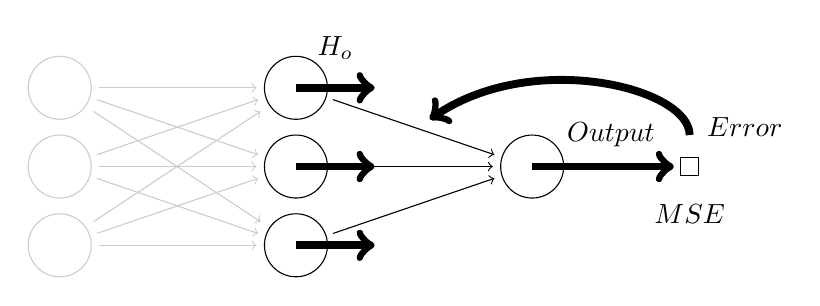
\begin{tikzpicture}
        
        \draw [draw={rgb:black,1;white,4}, ] (0.5,1) circle [radius=0.4];
        \draw [draw={rgb:black,1;white,4}, ] (0.5,0) circle [radius=0.4];
        \draw [draw={rgb:black,1;white,4}, ] (0.5,-1) circle [radius=0.4];

        \draw [] (3.5,1) circle [radius=0.4];
        \draw [] (3.5,0) circle [radius=0.4];
        \draw [] (3.5,-1) circle [radius=0.4];

        \draw [] (6.5, 0) circle [radius=0.4];

        \draw[draw={rgb:black,1;white,4}, ->] (1,1) -- (3,1);
        \draw[draw={rgb:black,1;white,4}, ->] (0.97,0.85) -- (3.02,0.15);
        \draw[draw={rgb:black,1;white,4}, ->] (0.93,0.7) -- (3.05,-0.7);

        \draw[draw={rgb:black,1;white,4}, ->] (0.97,0.15) -- (3.02,0.85);
        \draw[draw={rgb:black,1;white,4}, ->] (1,0) -- (3,0);
        \draw[draw={rgb:black,1;white,4}, ->] (0.97,-0.15) -- (3.02,-0.85);

        \draw[draw={rgb:black,1;white,4}, ->] (0.93,-0.7) -- (3.05,0.7);
        \draw[draw={rgb:black,1;white,4}, ->] (0.97,-0.85) -- (3.02,-0.15);
        \draw[draw={rgb:black,1;white,4}, ->] (1,-1) -- (3,-1);
        
        \draw[->] (3.97,0.85) -- (6.02,0.15);
        \draw[->] (4, 0) -- (6,0);
        \draw[->] (3.97, -0.85) -- (6.02,-0.15);
        
        \draw[->, line width=1mm] (3.5,1) -- (4.5,1);
        \draw[->, line width=1mm] (3.5,0) -- (4.5,0);
        \draw[->, line width=1mm] (3.5,-1) -- (4.5,-1);
        
        \draw[->, line width=1mm] (6.5,0) -- (8.3,0);
        
        \node at (7.5,0.4) {$Output$};
        \node at (4,1.5) {$H_o$};
        
        \node[draw] at (8.5,0) () {};
        \node at (8.5,-0.6) {$MSE$};
        \node at (9.2,0.5) {$Error$};
        
        \draw [->, line width=1mm] (8.5,0.4) .. controls (8.5,1) and (6.5,1.5) .. (5.2,0.6);
    \end{tikzpicture}
    \caption{Finding the error with mean squared error and sending it backwards.}
    \label{fig:backprop_one} 
\end{figure}

To actually train a neural network the weights between each layer has to be modified to reduce the overall error of the output. Gradient descent is used for this, where the partial derivatives for the error produced by a unit is calculated with respect to each of the connected weights.

For the neural network in figure \ref{fig:backprop_one}, the error from the output layer is first used to calculate the modifications for the weights between the hidden layer and the output layer. Then, the process is repeated for each of the hidden units. Three new errors is calculated, one for each of the hidden units. Finally, these errors are used to calculate the modifications for the weights between the input layer and hidden layer.

\begin{figure}[H]
  \centering

    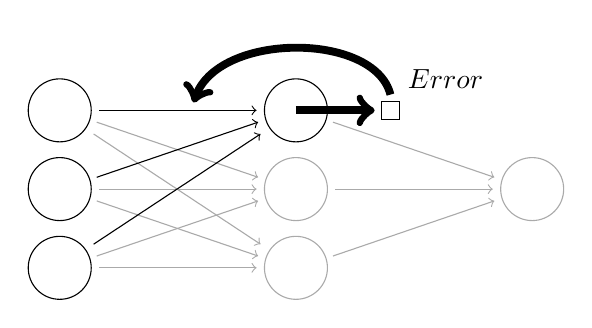
\begin{tikzpicture}
        
        \draw [] (0.5,1) circle [radius=0.4];
        \draw [] (0.5,0) circle [radius=0.4];
        \draw [] (0.5,-1) circle [radius=0.4];

        \draw [] (3.5,1) circle [radius=0.4];
        \draw [draw={rgb:black,2;white,4}, ] (3.5,0) circle [radius=0.4];
        \draw [draw={rgb:black,2;white,4}, ] (3.5,-1) circle [radius=0.4];

        \draw [draw={rgb:black,2;white,4}, ] (6.5, 0) circle [radius=0.4];

        \draw[->] (1,1) -- (3,1);
        \draw[draw={rgb:black,2;white,4}, ->] (0.97,0.85) -- (3.02,0.15);
        \draw[draw={rgb:black,2;white,4}, ->] (0.93,0.7) -- (3.05,-0.7);

        \draw[->] (0.97,0.15) -- (3.02,0.85);
        \draw[draw={rgb:black,2;white,4}, ->] (1,0) -- (3,0);
        \draw[draw={rgb:black,2;white,4}, ->] (0.97,-0.15) -- (3.02,-0.85);

        \draw[->] (0.93,-0.7) -- (3.05,0.7);
        \draw[draw={rgb:black,2;white,4}, ->] (0.97,-0.85) -- (3.02,-0.15);
        \draw[draw={rgb:black,2;white,4}, ->] (1,-1) -- (3,-1);
        
        \draw[draw={rgb:black,2;white,4}, ->] (3.97,0.85) -- (6.02,0.15);
        \draw[draw={rgb:black,2;white,4}, ->] (4, 0) -- (6,0);
        \draw[draw={rgb:black,2;white,4}, ->] (3.97, -0.85) -- (6.02,-0.15);
        
        \draw[->, line width=1mm] (3.5,1) -- (4.5,1);
        
        \node[draw] at (4.7,1) () {};
        \node at (5.4,1.4) {$Error$};
        \draw [->, line width=1mm] (4.7,1.2) .. controls (4.5,2) and (2.5,2) .. (2.2,1.1);


    \end{tikzpicture}
    \caption{Using error from the hidden units to calculate modification for the connected weights. The same process is repeated for the other hidden units.}
    \label{fig:backprop_two} 
\end{figure}


\subsection{Dropout}
\label{dropout}

Dropout is a technique used during training of a neural network. For a training sample, random units and all their connections are temporary dropped from the neural network \parencite{srivastava_dropout:_2014}. This means that the connections dropped will not be updated for the current training sample. 

\begin{figure}[H]
\centering
    \begin{subfigure}{1\textwidth} 
    \centering
        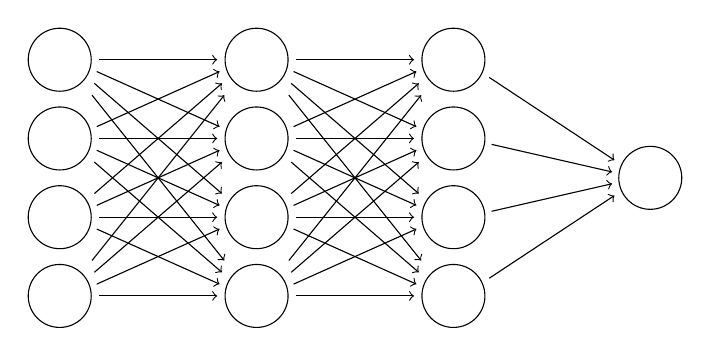
\begin{tikzpicture}

            \draw [] (-2.5,3) circle [radius=0.4];
            \draw [] (-2.5,2) circle [radius=0.4];
            \draw [] (-2.5,1) circle [radius=0.4];
            \draw [] (-2.5,0) circle [radius=0.4];

            \draw [] (0,3) circle [radius=0.4];
            \draw [] (0,2) circle [radius=0.4];
            \draw [] (0,1) circle [radius=0.4];
            \draw [] (0,0) circle [radius=0.4];

            \draw [] (2.5,3) circle [radius=0.4];
            \draw [] (2.5,2) circle [radius=0.4];
            \draw [] (2.5,1) circle [radius=0.4];
            \draw [] (2.5,0) circle [radius=0.4];
            
            \draw [] (5,1.5) circle [radius=0.4];
            
            
            \draw[->] (-2,3) -- (-0.5,3);
            \draw[->] (-2.03,2.85) -- (-0.47,2.15);
            \draw[->] (-2.06,2.7) -- (-0.44,1.30);
            \draw[->] (-2.09,2.55) -- (-0.41,0.45);
            
            \draw[->] (-2.03,2.15) -- (-0.47,2.85);
            \draw[->] (-2,2) -- (-0.5,2);
            \draw[->] (-2.03,1.85) -- (-0.47,1.15);
            \draw[->] (-2.06,1.70) -- (-0.44,0.30);
            
            \draw[->] (-2.06,1.3) -- (-0.44,2.7);
            \draw[->] (-2.03,1.15) -- (-0.47,1.85);
            \draw[->] (-2,1) -- (-0.5,1);
            \draw[->] (-2.03,0.85) -- (-0.47,0.15);
            
            \draw[->] (-2.09,0.45) -- (-0.41,2.55);
            \draw[->] (-2.06,0.30) -- (-0.44,1.7);
            \draw[->] (-2.03,0.15) -- (-0.47,0.85);
            \draw[->] (-2,0) -- (-0.5,0);
            
            
            \draw[->] (0.5,3) -- (2,3);
            \draw[->] (0.47,2.85) -- (2.03,2.15);
            \draw[->] (0.44,2.7) -- (2.06,1.30);
            \draw[->] (0.41,2.55) -- (2.09,0.45);
            
            \draw[->] (0.47,2.15) -- (2.03,2.85);
            \draw[->] (0.5,2) -- (2,2);
            \draw[->] (0.47,1.85) -- (2.03,1.15);
            \draw[->] (0.44,1.70) -- (2.06,0.30);
            
            \draw[->] (0.44,1.3) -- (2.06,2.7);
            \draw[->] (0.47,1.15) -- (2.03,1.85);
            \draw[->] (0.5,1) -- (2,1);
            \draw[->] (0.47,0.85) -- (2.03,0.15);
            
            \draw[->] (0.41,0.45) -- (2.09,2.55);
            \draw[->] (0.44,0.30) -- (2.06,1.7);
            \draw[->] (0.47,0.15) -- (2.03,0.85);
            \draw[->] (0.5,0) -- (2,0);
            
            
            \draw[->] (2.955,2.775) -- (4.545,1.725);
            \draw[->] (2.985,1.925) -- (4.515,1.575);
            \draw[->] (2.985,1.075) -- (4.515,1.425);
            \draw[->] (2.955,0.225) -- (4.545,1.275);
            
            
        \end{tikzpicture}
    \caption{}
    \label{fig:net_without_dropout}
    \end{subfigure}
    \begin{subfigure}{1\textwidth}
    \centering
        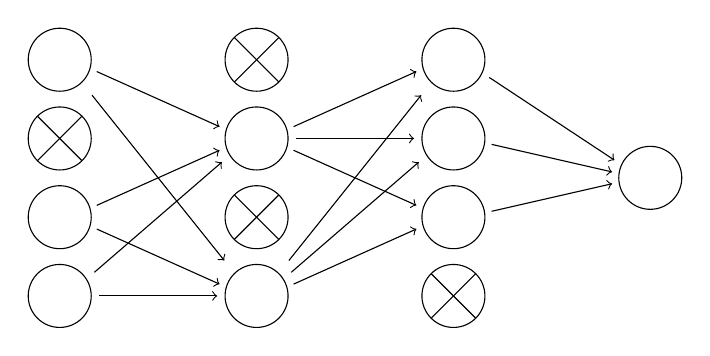
\begin{tikzpicture}
            \draw [] (-2.5,3) circle [radius=0.4];
            \draw [] (-2.5,2) circle [radius=0.4];
            \draw [] (-2.5,1) circle [radius=0.4];
            \draw [] (-2.5,0) circle [radius=0.4];

            \draw [] (0,3) circle [radius=0.4];
            \draw [] (0,2) circle [radius=0.4];
            \draw [] (0,1) circle [radius=0.4];
            \draw [] (0,0) circle [radius=0.4];

            \draw [] (2.5,3) circle [radius=0.4];
            \draw [] (2.5,2) circle [radius=0.4];
            \draw [] (2.5,1) circle [radius=0.4];
            \draw [] (2.5,0) circle [radius=0.4];
            
            \draw [] (5,1.5) circle [radius=0.4];
            
            \draw[-] (-2.78,2.28) -- (-2.22,1.72);
            \draw[-] (-2.78,1.72) -- (-2.22,2.28);
            
            \draw[-] (-0.28,3.28) -- (0.28,2.72);
            \draw[-] (-0.28,2.72) -- (0.28,3.28);
            
            \draw[-] (-0.28,1.28) -- (0.28,0.72);
            \draw[-] (-0.28,0.72) -- (0.28,1.28);
            
            \draw[-] (2.22,0.28) -- (2.78,-0.28);
            \draw[-] (2.22,-0.28) -- (2.78,0.28);
            
            
            \draw[->] (-2.03,2.85) -- (-0.47,2.15);
            \draw[->] (-2.09,2.55) -- (-0.41,0.45);
            
            \draw[->] (-2.03,1.15) -- (-0.47,1.85);
            \draw[->] (-2.03,0.85) -- (-0.47,0.15);
            
            \draw[->] (-2.06,0.30) -- (-0.44,1.7);
            \draw[->] (-2,0) -- (-0.5,0);
            
            
            \draw[->] (0.47,2.15) -- (2.03,2.85);
            \draw[->] (0.5,2) -- (2,2);
            \draw[->] (0.47,1.85) -- (2.03,1.15);
            
            \draw[->] (0.41,0.45) -- (2.09,2.55);
            \draw[->] (0.44,0.30) -- (2.06,1.7);
            \draw[->] (0.47,0.15) -- (2.03,0.85);
            

            \draw[->] (2.955,2.775) -- (4.545,1.725);
            \draw[->] (2.985,1.925) -- (4.515,1.575);
            \draw[->] (2.985,1.075) -- (4.515,1.425);
        \end{tikzpicture}
    \caption{}
    \label{fig:net_with_dropout}
    \end{subfigure}
\caption{Neural networks without (A) and with (B) dropout applied. The crossed circles are the dropped units.}
\label{fig:dropout_comparison}
\end{figure}

The purpose of dropout is to reduce the chance of overfitting a neural network. A neural network is overfitted when it is too closely related to the training samples, and not being as generalized as possible. An overfitted neural network will give good results if tested with the training data, but might fail on new data that the neural network has not seen before. Underfitting is the opposite of overfitting, and describes a too generalized network. %On the other side, a neural network is underfitted when it is too generalized. In this case the neural network would ignore 

In a paper by Srivastava et al. from 2014 \cite{srivastava_dropout:_2014}, classifiers and neural networks trained with and without dropout applied is compared using standardized data sets. These data sets covers several areas, including vision, speech and text. In every comparison, neural networks with dropout was ranked high, if not highest.

\subsection{Common problems}
\label{vanishing-gradient}
\label{exploding-gradient}
\label{dead-neurons}
In artificial neural networks there are issues that optimization algorithms must overcome. The first issues to address is the vanishing and exploding gradient. These issues typically occur in deep feedforward- and recurrent networks (these types are described in the next sections). The common factor is that both types of artificial neural network generate long computational graphs. To explain this problem further, some mathematics is required.

A square matrix $A$ with $n$ linear eigenvectors $q_i (i=1..n)$ can be factorized as
\begin{equation} \label{eqn:mat_decomp}
    A=Q diag(\lambda) Q^{-1} 
\end{equation}
In equation \ref{eqn:mat_decomp} $A$ is our original matrix, $Q$ is an $nxn$ matrix where each column is an eigenvector $q_i$ and $diag(\lambda)$ is a diagonal matrix of eigenvalues. If we do this multiplication $t$ times, it only changes the number of times the diagonal matrix is multiplied. \cite{weisstein_eigen_????}
\begin{equation} \label{eqn:mat_decomp_t}
    A^{t} = Q diag(\lambda)^{t} Q^{-1}
\end{equation}
Both the vanishing and exploding gradient issues originate from the scaling according to the diagonal matrix with eigenvalues $diag(\lambda)$, with repeated multiplication by $A$. Vanishing gradient makes it difficult to find out in which direction parameters should move in order to move the cost function. While exploding gradients makes learning unstable. \cite{goodfellow_deep_2016}

Another issue with artificial neural networks is "dead" neurons (units), and is a direct cause of using ReLU. ReLU is widely used to not get caught in between gradient issues, however, it can cause weights to be updated in a way that makes the neuron unable to activate again. This is an irreversible consequence of setting the learning rate too high.\cite{_cs231n_????}
 % Må forklare mer her?

\section{Feedforward neural networks}
% 
Feedforward neural networks, also referred to as deep feedforward networks or multilayer perceptrons (MLPs), are the most common deep learning models. The example network in figure \ref{fig:single_layered_neural_network} is a feedforward neural network. The ultimate goal of these networks is to approximate some function $f$, for example a task to classify (map) an input $x$ to a specific class $y$. In mathematical notation this can be written as $y = f*(x)$. The networks mapping is defined as $y = f(x,\theta)$ where $\theta$ is learned in a way to approximate $f$ the best way. Goodfellow et al. \cite{goodfellow_deep_2016}[p.~163] explains why networks such as these are called feedforward.

\begin{displayquote}[\cite{goodfellow_deep_2016}]
\textit{These models are called feedforward because information flows through the function being evaluated from x, through the intermediate computations used to define f, and finally to the output y. There are no feedback connections in which outputs of the model are fed back into itself.}
\end{displayquote}

\subsection{Convolutional networks}

Convolutional networks \cite{lecun_generalization_1989} is also often referred to as convolutional neural networks or CNNs. CNNs are specialized for processing data that has a known typology. Examples includes images, which is a 2D-grid of pixels and say time series data. In this attempt to get some accurate classifications for handwritten mathematics we are both using images and sequential data. The reason that CNNs are actually called a CNN is because they use a convolution, which is a mathematical operation.

\begin{displayquote}[\cite{goodfellow_deep_2016}]
 \textit{Convolutional networks are simply neural networks that use convolution in place of general matrix multiplication in at least one of their layers.}
\end{displayquote}
To understand this further, the convolution operation needs to be explained. A convolution can be explained as an operation on two functions with real-valued arguments. 

% TRENGER VI EKSEMPEL? VELDIG LIKT GOODFELLOW
% TODO Trenger review; håv
Deep Learning by Goofellow, Bengio and Courville explains a convolution with an example: we are tracking the location of a spaceship with a laser. Our laser is feeding us a single output x(t), which reads the position of the spaceship at time t. Now if the laser is noisy we may read data that could be unrepresentative. Thus, we could need some sort of average function. In addition, we would also like to specify that the most recent recordings are the most important ones. This is solvable using weights, where $w(a)$ is the weight function and $a$ is the age of a measurement. \cite{goodfellow_deep_2016}

\begin{figure}[H]
    \label{eqn:conv}
    \begin{equation}
    s(t) = \int x(a)w(t-a)da
    \end{equation}
    \caption{\cite{goodfellow_deep_2016}[p.~322] Example convolution which averages sensor readings and weights the most recent sensor readings. w(a) is the weighting function, x(t) is the position of the spaceship at time t. The result of this is a new function s, which gives us a smoothed estimate}
\end{figure}

\begin{figure}[H]
    \label{fig:conv_asterisk}
    \begin{equation}
        s(t) = (x*w)(t)
    \end{equation}
    \caption{Asterisk notation of a convolution.}
\end{figure}
% TRENGER VI EKSEMPEL? VELDIG LIKT GOOFELLOW
The first and second argument is often called the input and kernel, while the output is called the feature map. In the example with lasers $x$ would be our input and $w$ would be the kernel. % Eksempel på feature map ?
% Diskret notasjon
In a perfect world the laser would be able to provide real-time measurements, however, this is not realistic. Often readings are discretized, that means that a new reading will arrive at a given interval, an example of this could be a new reading every second. This would eventually lead to $t$ being an integer, and since both $x$ and $w$ is dependent on $t$ we end up with a discrete convolution. \parencite{goodfellow_deep_2016}
\begin{figure}[H]
    \label{fig:disc_conv}
    \begin{equation}
        s(t) = (x*w)(t) = \sum_{a=-\infty}^{\infty} x(a)w(t-a)
    \end{equation}
    \caption{Definition of the discrete convolution. \cite{goodfellow_deep_2016}[p.~323]}
\end{figure}

For two-dimensional inputs, two-dimensional kernels are used. These are commutative:
%For two-dimensional inputs, there is two-dimensional kernels, which is commutative:

\begin{figure}[H]
    \label{fig:disc_conv2d}
    \begin{equation}
        S(i,j) = (I*K)(i,j) = \sum_{m} \sum_{n} I(m,n)K(i-m,j-n)
    \end{equation}
    \begin{equation}
        S(i,j) = (K*I)(i,j) = \sum_{m} \sum_{n} I(i-m,j-n)K(m,n)
    \end{equation}
    \caption{\cite{goodfellow_deep_2016}[p.~323] The two dimensional kernel in both it's original form in addition to the version with the flipped kernel. The last version is a result of flipping the kernel relative to it's input.}
\end{figure}

% SJEKK OM VI TRENGER KOMMUTATIVE ALTERNATIVET. 
The actual function that usually exists in machine learning libraries is cross-correlation. Cross-correlation is the same as a convolution without flipping the kernel and is often referred as convolution.

\begin{figure}[H]
    \begin{equation}
        S(i,j) = (K*I)(i,j) = \sum_{m} \sum_{n} I(i+m,j+n)K(m,n)
    \end{equation}
    \label{fig:cross_corr}
    \caption{The cross-correlation function. \cite{goodfellow_deep_2016}[p.~324]}
\end{figure}

Sparse interactions, connectivity or weights is a result of making the kernel smaller than the input. Even if an image has many thousands of pixels it is possible to extract small crucial features using smaller kernel sizes.

\begin{figure}[H]
    \centering
    \includegraphics[width=\textwidth]{Assets/Chapter2_Theory/kernel_applied.png}
    \caption{\cite{nielsen_neural_2015} This figure shows how a convolution layer works with a 5x5 kernel, also referred to as a filter or feature detector. In this example, our input is 28x28, if we apply a 5x5 kernel we will end up with 24x24 units in the hidden layer. Available from http://neuralnetworksanddeeplearning.com/images/tikz45.png, 23.04.2018}
    \label{fig:kernel_applied}
\end{figure}

%In summary the convolutional layer accepts a volume of size \textbf{$W_1$ x $H_1$ x $D_1$}. In addition to a volume, it needs to provide four \gls{hyperparameters}. These \gls{hyperparameters} are the number of filters \textbf{K}, their spartial extent \textbf{F}, the stride \textbf{S} and the ammount of zero padding \textbf{P}. 
A convolutional layer has typically three stages, the first is to do the convolutions as illustrated in \ref{fig:kernel_applied}, these are linear activations. When all the convolutions are done, they are passed through a nonlinear activation function. An example of a \gls{nonlinear} activation function is the sigmoid function from \ref{eqn:sigmoid}. Furthermore this stage is often referred to as the detector stage.

The last stage of the a typical convolutional layer is when we apply a pooling function to further modify the output \parencite{zhou_computation_1988}. A pooling function is able to replace the output of a small area with a summary of the nearby outputs. An example of a pooling function is the max pooling, which function uses a pooling unit with a specified size, for example 2x2. The pooling unit in a max pooling function simply outputs the maximum activation of it's region (2x2). A max pooling function with this pooling unit would turn 24x24 units to 12x12 units. \cite{goodfellow_deep_2016} \cite{nielsen_neural_2015}

\section{Recurrent neural networks}

Recurrent neural networks, also referred to as RNNs  are neural networks which can process sequential data\parencite{rumelhart_learning_1986}. While CNNs are specialized on analyzing grid like data, such as images or videos, RNNs are more specialized on processing sequential data. The idea behind RNNs is to share parameters in different parts of a model. Sharing parameters makes it possible to use the model on data with variable length. \begin{displayquote}[\cite{goodfellow_deep_2016}]
 \textit{Such sharing is particularly important when a specific piece of information can occur at multiple positions within the sequence.}
\end{displayquote}
Furthermore, an artificial neuron or computing unit is not only determined by it's activations in previous layers, it is now possible for an artificial neuron or computing unit to be determined by it's own activation earlier. \parencite{goodfellow_deep_2016} \cite{nielsen_neural_2015}

%Data provided by the CROHME competitions is sequential ink coordinates as illustrated in listing \ref{lst:InkML_ex}. Thus, the principle of information sharing is quite significant in this projects case as well. 
% TODO sjekk om dette er bra eksempel. Kanskje bruk heller at skal man lære et språk må man lære alle regler for hver posisjon i en setning for eksempel, noe som gjør treningen og oppgaven veldig vanskelig.
% konkluderte med at det ikke er et veldig bra eksempel, skriv enten om eller dropp. [Drop]

\subsection{Long short-term memory}
\label{theory-LSTM}
Long short-term memory unit is a type of computational unit often used in recurrent neural networks. LSTM networks were introduces in 1997 by Sepp Hochreiter and Jürgen Schmidhuber \cite{hochreiter_long_1997}. LSTM networks has been improved in further research, for instance by giving the network the ability to forget \cite{gers_learning_1999}. These units can be utilized to keep important information over time, as opposed to traditional recurrent units, by adding new information on top of old state and not overriding it for each time step. This is described in a paper by J. Chung et al. \cite{chung_empirical_2014}.

\begin{displayquote}[\cite{chung_empirical_2014}]
    \textit{Intuitively, if the LSTM unit detects an important feature from an input sequence at early stage, it
    easily carries this information (the existence of the feature) over a long distance, hence, capturing
    potential long-distance dependencies.}
\end{displayquote}

LSTM layers typically consist of a several computational units. These will be referred to as \textit{memory cells}, and a collection of one or more cells will be referred to as \textit{memory blocks}. The input at the current timestep $t$ is notated with $x$, the output of the cells are notated by $h$, and the block's state is notated as $C$.

A key part of an LSTM memory block is the Constant Error Carousels (CEC) \cite{gers_learning_1999}, also known as state. This is visualized as the horizontal line in the top part of the figure below. The state flows through all cells in a memory block, and the state eventually determines the cell's output.

Each memory cell includes several gates, which are used to decide what the network should remember. These gates determine how the input should influence the state of the memory block. This is done through filters, which are combinations of a sigmoid activation function and a pointwise multiplication. These filters are known as gates. A typical LSTM memory cell has three gates, an input gate, output gate and a forget gate.

\begin{figure}[H]
    \centering
    \includegraphics[width=\textwidth]{Assets/Chapter2_Theory/LSTM3-chain.png}
    \caption{Model of a memory block with three memory cells. The center cell includes a visualization of the different parts of the cell, and how the information flows inside the cell. The cell's input values are the current state of the memory block $C_{t-1}$ (top left), the output of the previous cell $h_{t-1}$ (bottom left), and  the current input value $x_t$. The upper line is the memory block's state, which flows through each cell of the block. The yellow squares are neural network layers with a specified activation function. \cite{_understanding_2015} Available from http://colah.github.io/posts/2015-08-Understanding-LSTMs/img/LSTM3-chain.png at 10-05-2018.}
    \label{fig:lstm_cells}
\end{figure}

The first gate in the memory cell is the input gate. This gate is notated as the combination of the sigmoid layer and the pointwise multiplication in the top left of the cell. This gate decides how much the previous cell's output $h_{t-1}$, and this timestep's input $x_t$ should influence the current state. The output of the sigmoid function is multiplied with the previous state $C_{t-1}$. If the output is 0, everything should be forgotten, and if the output is 1, everything should be remembered. 

The following layer with sigmoid activation determines how much of the current input should influence the memory state. This process is similar to the input gate. The layer noted by the $tanh$ activation function decides what should be remembered. The output of the pointwise multiplication between the sigmoid and tanh layer, is then added to the state.

The output of the memory cell is a filtered version of the current state, as seen top right in \ref{fig:lstm_cells}. The cell's state is run through a $tanh$ function, to squish the values in the range $[-1, 1]$, then the output is filtered through the output of the sigmoid function, similar to how state was removed and added in the previous steps. 

The sequential nature of these memory blocks makes LSTM networks good for predicting sequencial data. In pratice, most of the information we encounter is not needed for future predictions. By using gates, the LSTM network is able to decide which information should be remembered and to which scale the previously remembered information should influence future decisions. \cite{gers_learning_1999}\cite{_understanding_2015}

\subsection{Gated Recurrent Unit}

%Ny setning:     GRU cells' advantage over LSTM is that it includes the same functionality in a less complex cell
%Gammel setning: GRU has the same capabilities of keeping important information over time using gates, however without use of the LSTM's memory cells.

Gated Recurrent Unit is often referred to as GRU. It was recently proposed in 2014 by Cho et al. \cite{cho_learning_2014}, as an alternative to LSTM. GRU cells' advantage over LSTM is that it includes the same functionality in a less complex cell. This makes a GRU unit cheaper computationally, and has shown to outperform LSTM on models with fixed parameters \cite{chung_empirical_2014}. 

\begin{figure}[H]
    \centering
    \includegraphics[width=\textwidth]{Assets/Chapter2_Theory/GRU-cell.png}
    \caption{A model of a Gated Recurrent Unit $h_{t-1}$ is the output of previous cell, $h_t$ is the output of current cell. $z_t$ is the output from the update gate. $r_t$ is the output of the reset gate. $x_t$ is the input at current timestep. Available at https://cdn-images-1.medium.com/max/800/1*6eNTqLzQ08AABo-STFNiBw.png (10-05-2018) \cite{kostadinov_understanding_2017}}.  
    \label{fig:gru-single-cell}
\end{figure}

The GRU cell calculates a temporary state from a combination of the previous state and the current input. The temporary state will be notated as $h_{tmp}$.

$h_{tmp}$ is calculated by adding the input at a timestep $x_t$ to a part of the previous state $h_{t-1}$. The influence of $h_{t-1}$ on $h_{tmp}$ is decided by the reset gate, $r_t$. This addition is then the input to a layer with a $tanh$ activation function, and results in $h_{tmp}$.

To calculate the output of the GRU cell, the cell needs to decide how much of the previous state it is going to keep. This is decided by the update gate $z_t$. Through a element-wise multiplication of $z_t$ with $h_{t-1}$, only the important parts of the previous state is kept. $h_{tmp}$ is multiplied element-wise with $1 - z_t$, and thereby the state removed from previous state is substituted with the state calculated in the current cell.

It is important to remember that the different gate's outputs is a value in the range $[0, 1]$, therefore if $z_t = 0$ then $1 - z_t = 1$

If the update gate is 0, $z_t = 0$, and none of the previous state should be kept. This leads to $1 - z_t = 1$, and the all the current state will be kept. On the other hand, if $z_t = 1$, the cell's output will equal the previous cell's output $h_{t-1} = h_t$, and the current input will not influence the output of the cell ($1 - z_t = 0$). \cite{kostadinov_understanding_2017} 

\chapter{Technology and method}
\lhead{\emph{Technology and method}}

% Hardkoding og logikk for søk etter kontekst
% 

\section{Introduction}
% Var vi limited til å følge matistikk?
In this chapter the technology and methods applied in this project is reasoned. The project was at no point limited to follow Matistikk, but for the sake of simplicity and engineering flexibility tools which both provided good results in short time and if it were to be implemented in Matistikk, a Python solution was preferable.
% TODO Sjekk om jeg ikke prater opp igjen mange ganger


\section{Technology}
The choice of technology was highly influenced by the nature of the project assignment, if the goal was to create a module for an existing Django application, Python was already the obvious choice. Eventually the project drifted in the way of a proof of concept, Python came out even further as the obvious choice. The reason why Python is the obvious choice in this case, is the ability to go from idea to a working prototype in the fastest way possible. In addition to productivity Python has a lot of mature libraries, in the nature of working towards a proof of concept, one would need stable, tested and well documented libraries. We found especially Keras \parencite{chollet_keras_2015} to be a perfect fit for our task, which is a library that makes TensorFlow or some other machine learning library easier to use.\\
\quad
The choice of back end and processing tool was now chosen, Keras backed by TensorFlow is an extremely feature-rich combination. Since the project went in the way of a proof of concept we needed some graphical user interface in which we could collect data, present statistics and so forth. The selection of front end was determined by the project assignment. Since Matistikk is web-based, we found it quite natural to go with some simple HTML, Css, JavaScript and Tornado. Tornado is a simple library to build web servers in Python.

\section{Communication and dataflow}
The foundation was quickly made, that led to an classic client/server approach. Already in the first weeks of the project Keras and deep learning was our focus.% dårlig setning...
The progress made was not only based on our own experimentation. Articles and projects posted was quickly digested and learned from. CROHME gave the project it's desirable data and insight into the assignment. CROHME provided both tools and  sequential data in InkML files, see listing \ref{lst:InkML_ex} for an InkML example file.\\
Even with the new discovered data, the research still continued.  Lu and Mohan \cite{lu_recognition_2015} and Thoma \cite{thoma_-line_2015} inspired the work made in this project. The majority of data at that stage was sequential, a decision was made to use a \gls{WebSocket} to handle front to back end communication. For the sake of simplicity, it was also implemented a way to do this over a simple http post request as an alternative to the WebSocket implementation. Doing it this way created a simple, but solid foundation for the engineers behind Matistikk to do it the way they wanted. \\
After discussion with our project owners, we were drawn to the direction of using a http post request. The test application also does not think about the amount of data it sends per classification request. If the canvas is changed, it still re-sends the entire buffer. This is both to easy re-evaluate the buffer, but in addition this can trigger changes in the segmentation process, which can eventually lead to a different classification.

\section{The recognition system} % TODO vurder om dette er for nært resultat kapittelet. SE MAL
The recognition system consists of both some "hard-coded" logic and the neural network. As stated in chapter 2.1, handwriting recognition includes several steps required to classify correctly. The "hard-coded" logic solves the segmentation issue in an elementary way, but it is quite vulnerable to noisy input. In addition to segmentation we do a whole lot of prepossessing to make sure our actual data flowing from our front end to our back end is roughly the same size format, data type and so forth. % TODO Insert a simple diagram of our system

\section{Artificial Neural Network}
Artificial neural networks in image recognition is often to be found in tutorials. Since the project engineers had no prior experience with artificial neural networks it was necessary to experiment with different types of neural network and data. The MNIST data set consists of handwritten digits which is available in Keras. The amount of thorough tutorials on the MNIST data set inspired the project in new aspects. At that time, there was made a decision to use CNNs to handle the recognition problem. This meant that all the sequential data must be converted into images. \\ This was a decision that turned out to work as desired, it was not a choice that led to success. But the issue was not more focused on handling segmentation and applying different techniques to obtain good accuracy. After some experimentation with CNNs, attempts at getting it done with RNNs was started. The project went into a hard period, where we were battling variable length input and at the same time we felt that our working solution would not improve. % Trenger review..

\section{Classification model}

% The neural network 

\section{Architecture}



\section{Image data}
When deciding on the image format it was clear that the best approach was to resemble an already existing data set in order to obtain more data. Experimenting on the MNIST data made the project engineers explore possibilities to convert our InkML data to grey scale images in the same format as MNIST data. This, of course was no straight forward procedure, after several tries over a couple of weeks it was decided to go forward with generating bitmaps. Generating BMPs was a much simpler task, and luckily we found BMPs that were of handwritten mathematical symbols.

\subsection{Preprocessing}
\begin{figure}[H]
    \centering
    \includegraphics{Assets/Chapter3_Method/sqrt_before_preprocessing.png}
    \caption{A square root which has not been thorough preprocessing.}
    \label{fig:sqrt_not_processed}
\end{figure}

\begin{figure}[H]
    \centering
    \includegraphics{Assets/Chapter3_Method/sqrt_after_preprocessing.png}
    \caption{A square root which has been through preprocessing.}
    \label{fig:sqrt_processed}
\end{figure}

\begin{figure}[H]
    \centering
    \includegraphics{Assets/Chapter3_Method/sqrt_image.png}
    \caption{The resulting square root from the preprocessing done in previous steps.\\The generated image is 26x26 pixels.}
    \label{fig:sqrt_img}
\end{figure}

\section{Segmentation}
Since the project initially went for a solution with a CNN, we had to separate the system into different tasks. The reason behind this is that the CNN itself, in our solution should solely work on the classification of a symbol. Since our assignment is to handle symbols and expressions, we then need to extract single symbols from multiple symbols or expressions.\\
This specific task was and is the most critical in order to get correct recognition with a CNN. If the segmentation turned out wrong, the classification would be handed bad data which makes a correct classification unlikely.\\ To solve the segmentation issue different approaches was attempted, among those were object localization and detection, with bounding boxes to easily detect symbols which consists of multiple strokes or traces. This idea of object detection was quite good and would have, if successful made the rest quite easy in comparison.\\ The attempts made on object detection was unsuccessful, we were getting results, but they were not proving to be better than solving it with a much simpler algorithm which did not require machine learning in the first place. 


%This decision turned out to be very wise. Eventually new data was discovered, this was from the CROHME competitions as well, but it had been turned into images for us.% CITE KAGGLE CROHME => BILDER


\section{Interpretation and context search} % SKRIVER LITT OM DETTE I \section{Segmentation}
% Har skrevet om at vi hardkodet segmentering, så ta det derfra. (fins i \section{Segmentation})



The interpretation system consist of a recursive search function and a set of fixed rules to determine the context of how the symbols fit together. This system all the symbols 

[Model of the overall architecture]





\section{Project process}
The project process in terms of software engineering methodology had been a mix between multiple concepts and paradigms. In the early stages of the project methodologies from the agile world were mostly used, such as pair programming. In the early stages of the project, we followed to some extent a methodology called Lean startup. Lean startup focuses on creating a minimal viable product, often referred to as \gls{MVP}. When the MVP was out, constructive discussions with the product owners about what they liked and what they did not like. This assignment required a lot of curiosity and as project participants, one could never go hungry. This is why, at some stage the project split in different ways, we were continuously working on improving the product, but the main focus was on how we could do the recognition itself better.


\section{Teamwork and roles}
Since the project is more of a research based project, it was not easy to define a simple structure as more common in software engineering projects. Although, a simple structure was created to get the MVP up, this was Even on front end, Torkil and Håvard on back end. \\ % TODO Fortsett dette, se MAL
With the MVP up, the project quickly took principles from agile thoughts and methodologies, even though we could not plan an entire sprint to detail, we had a stand-up meeting, or quick recap of the progress and issues. This enabled a dynamic and flexible structure which led us to working together quite effective, when the project stagnated, we would quickly help each other out. When it came to exploring the potential behind RNN it was simply not easy to grasp how to approach this issue in order to classify correctly. This took one of the project engineers several weeks to get going and when the attempts were up for evaluation and the other project engineers understood the issue, a better solution and RNN was created. % Trenger kanskje ikke?


%\cite{_tensorflow_????}





\chapter{Results}
\lhead{\emph{Results}}

\section{Scientific results}
This section will contain data, visualizations and results from the work associated with the scientific problem described in section \ref{problem_definition}.

In order to evaluate the different ANN models against each other, each model classified three different datasets in every iteration. Every training session therefore includes three different accuracy's, where each accuracy is calculated as correct predictions divided by total predictions.

The first dataset is the training set. This dataset consists of a large subset of data gathered from the CHROME dataset (90\%), and is the data the models used as training data. This dataset is labelled as \textit{train} in the accuracy graphs below. % små avsnitt? evt slå sammen?

The second dataset is the validation set, also called the test set. This dataset consists of the last 10\% of data from the CHROME dataset. None of the data in the validation set was used during training, and this data is therefore a good representation for how the model performs on unseen data. This dataset is labelled as \textit{test} in the accuracy graphs below.

The third dataset is a set of real data gathered from the example website, with symbols written by three different people. This dataset is used to give an indication of the correctness of the preprocessing, as well as how the model responds to data from different sources. The real dataset was an important inclusion because the main goal of this assignment was to produce good results under circumstances simulated by the example website. Notice that this dataset included a few mislabelled data points, contained only about three hundred data points, and includes only a subset of all the classes. The dataset is therefore only used as an indication of the accuracy on real data. This dataset is labelled as \textit{real} in the accuracy graphs below.

%TODO her må vi forklare hva train test og real er.
\begin{figure}[H]
    \centering
    \includegraphics[width=0.8\linewidth]{Assets/Chapter4_Result/CNN_40_epoch.png}
    \caption{Training accuracy from the CNN model with 44000 data points evaluated for 40 epochs.}
    \label{fig:CNN_44000}
\end{figure}
\begin{figure}[H]
    \centering
    \includegraphics[width=0.8\linewidth]{Assets/Chapter4_Result/RNN_40_epoch.png}
    \caption{Training accguracy from the RNN model with 44000 data points evaluated for 40 epochs.}
    \label{fig:RNN_44000}
\end{figure}

\begin{figure}[H]
    \centering
    \includegraphics[width=.8\linewidth]{Assets/Chapter4_Result/Combined_CNN_and_RNN_40_epoch.png}
    \caption{Training accuracy from the combined CNN and RNN model with 44000 datapoints. Evaluated for 40 epochs.}
    \label{fig:combined_CNN_RNN_44000}
\end{figure}

The tables below show the same data in tabular form. Each row is a snapshot of the different models' accuracy in percent at specific epochs. 

Table of the \textit{train} dataset.
\begin{figure}[H]
    \centering
        \begin{tabular}{| p{2cm} | p{3cm} | p{3cm} | p{3cm} |}
    \hline
    Epoch & \textbf{CNN} & \textbf{RNN} & \textbf{Combined} \\ \hline
    10 & 97.66 & 93.99 & 97.53 \\ \hline
    20 & 98.43 & 94.87 & 98.08 \\ \hline
    30 & 98.81 & 95.62 & 98.44 \\ \hline
    40 & 98.86 & 95.95 & 98.46 \\ \hline
    \end{tabular}
    \caption{Snapshot of accuracy in percent on the train dataset for all models at epoch number 10, 20, 30 and 40}

    \label{fig:table_train_dataset}
\end{figure}

Table of the \textit{test} dataset.
\begin{figure}[H]
    \centering
    \begin{tabular}{| p{2cm} | p{3cm} | p{3cm} | p{3cm} |}
    \hline
    Epoch & \textbf{CNN} & \textbf{RNN} & \textbf{Combined} \\ \hline
    10 & 95.48 & 96.82 & 98.07 \\ \hline
    20 & 95.29 & 97.31 & 98.13 \\ \hline
    30 & 95.98 & 97.46 & 98.13 \\ \hline
    40 & 96.51 & 97.35 & 98.28 \\ \hline
    \end{tabular}
    \caption{Snapshot of accuracy in percent on the test dataset for all models at epoch number 10, 20, 30 and 40}
    \label{fig:table_test_dataset}

\end{figure}

Table of the \textit{real} dataset.
\begin{figure}[H]
    \centering
    \begin{tabular}{| p{2cm} | p{3cm} | p{3cm} | p{3cm} |}
    \hline
    Epoch & \textbf{CNN} & \textbf{RNN} & \textbf{Combined} \\ \hline
    10 & 89.75 & 88.99 & 94.12 \\ \hline
    20 & 88.24 & 94.88 & 96.20 \\ \hline
    30 & 92.41 & 93.93 & 95.83 \\ \hline
    40 & 91.08 & 94.50 & 96.02 \\ \hline
    \end{tabular}
    \caption{Snapshot of accuracy in percent on the real dataset for all models at epoch number 10, 20, 30 and 40}
    \label{fig:table_real_dataset}

\end{figure}

\section{Engineering results}
This section will contain how our example project/proof of concept has turned out in terms of goals set in earlier stages of the project. The evaluation of engineering result is based on goals set in meetings with the product owners. % Resultat fra tester skal være lagt her

The product was intended to be a proof of concept application, with functionality for recognizing handwritten mathematical symbols. In addition, it was meant to be used as a module to enhance Matistikk's functionality. Therefore, the product had to be easily integrable to the already existing Matistikk. 


\begin{figure}[H]
    \centering
    \includegraphics[width=\textwidth]{Assets/Chapter4_Result/predictor_example.png}
    \caption{Example of the graphical user interface, with an HTML5 canvas. The result is shown at the top right corner in human readable form. Directly below is the corresponding \LaTeX script, which can be useful for further use in other APIs. The graph on the right contains the classification probabilities for either a chosen symbol or the latest drawn.}
    \label{fig:predictor_example}
\end{figure}

The back- and front end are developed as two separate products. These can be integrated independently into a larger system. An example implementation of this is deployed on Heroku, a cloud application platform.

Results from the algorithms behind segmentation and context was not easily measurable. They are however discussed in chapter \ref{engineering_results}.

\section{Administrative results}
Administrative results are the results of planning, implementing, researching and concluding the work done in this project. 

Due to the high uncertainty in the assignment, the planning had to be done in a dynamic process continuously through the project. After each small period it was necessary to do a retrospective, to learn from mistakes and further improve the project flow and productivity. Incorporating iterations and reviews into the project flow enhanced the ability to respond to changes and new goals. Modern Agile principles were followed during the project, and was a good fit for a research based assignment. Detailed planning was achievable when developing the foundation of the web-based system. 


\chapter{Discussion}
\lhead{\emph{Discussion}}

\section{A Section}

\subsection{A Subsection}


\chapter{Conclusion and further work}
\lhead{\emph{Conclusion and further work}}
Classifying handwritten mathematical symbols and expressions is a challenging task, where each step in the recognition process is critical and vulnerable in its own way. 

The results confirmed that a combination of convolutional and recurrent networks outperformed both networks individually. However, these results are confined to our dataset and models.  

From experimentation with different data formats, it is likely that keeping the sequential information from the digital drawings is an important factor in getting good accuracies. By combining both the static information from the finished symbol, and information about how the symbol was drawn, a network was able to find features resulting in high accuracies on a relatively small dataset.

In order to best classify an image, it seems that the sequential data contains more features that an RNN could extract than a CNN model could through static image data. Individually the recurrent network had better accuracy than the CNN, however, since the combined model achieved even better results, it is likely that both formats include different information, both important for the final classification.

\section{Further Work}

A pure recurrent neural network would have been exciting to see and compare results with. During the project there was a constant search for improvements, with enough data it is not unrealistic to see a recurrent neural outperform it's competitors, not just in classification accuracy, but in segmentation and extending the symbol bank. It is worth to mention though, that a recurrent neural network is primarily powerful when trained with sufficient amount of data. A standalone recurrent neural network would need some help to handle the different contextual relations between symbols.

Sequential data contains information which could be used to enhance segmentation, for example timestamps. Some of the InkML data contained timestamps between traces, that could be utilized to enhance the segmentation. For this to work, one would need large quantities of data where the timestamps are preserved.

Both the bounding box approach and using machine learning for context would also be worth exploring more. A solution including these techniques could result in a more general solution, and make it easier to extend both the symbol bank and contextual understanding.

Regarding improvements in the currently produced models, there is still a lot of experimentation to be done. Trying different learning rates, safeguarding against dead neurons and different model architectures are all areas that could be changed to increase accuracy. Making use of state-of-the-art models, and retraining on this specific dataset, is another untested approach that could have increased the accuracy. 



%% ----------------------------------------------------------------
% Now begin the Appendices, including them as separate files

\addtocontents{toc}{\vspace{2em}} % Add a gap in the Contents, for aesthetics
\backmatter
%% ----------------------------------------------------------------
%% ----------------------------------------------------------------
\printbibliography

\clearpage
\appendix % Cue to tell LaTeX that the following 'chapters' are Appendices
%\renewcommand\thechapter{}
%\renewcommand\thesection{\arabic{section}}
%\chapter{Appendix}
%\SuspendCounters{Chapter}
%\thispagestyle{plain}


%\section{System documentation}
%\includepdf[ pages=1, width=\textwidth]{Appendices/systemdokumentasjon.pdf}
%\includepdf[ pages=2-, width=\textwidth]{Appendices/systemdokumentasjon.pdf}
%\input{Appendices/AppendixB} % Appendix Title

%\input{Appendices/AppendixC} % Appendix Title


% END
\end{document}